% !TeX program = tectonic
% !TeX encoding = UTF-8
\documentclass[conference]{IEEEtran}

\usepackage[utf8]{inputenc}
\usepackage[T1]{fontenc}
\usepackage{amsmath,amssymb,amsfonts}
\usepackage{amsthm}
\usepackage{graphicx}
\usepackage{textcomp}
\usepackage{xcolor}
\usepackage{booktabs}
\usepackage{multirow}
\usepackage{array}
\usepackage{hyperref}
\usepackage{cleveref}
\usepackage{algorithm}
\usepackage{algorithmic}
\usepackage{microtype}

\hypersetup{
  colorlinks=true,
  linkcolor=blue!55!black,
  citecolor=blue!55!black,
  urlcolor=blue!55!black,
  pdftitle={Certify, Then Repair: Exact Worst-Case Guarantees for Recurrent Policies Trained Against Strong Teachers},
  pdfauthor={Starlyn Eliezer Rosario Reyes},
  pdfkeywords={reinforcement learning, optimal-play training, minimax, tie-breaking, worst-case certification, certificate-guided repair, dataset aggregation, distribution shift, Bayes-adaptive control, reproducibility, tic-tac-toe},
  pdfsubject={Certification and repair of game-playing agents against tied optimal teachers}
}

\newcommand{\R}{\mathbb{R}}
\newcommand{\E}{\mathbb{E}}
\newcommand{\ie}{\textit{i.e.}}
\newcommand{\eg}{\textit{e.g.}}
\newcommand{\etal}{\textit{et al.}}
\newcommand{\DR}{\text{DR}}

\newtheorem{proposition}{Proposition}
\newtheorem{lemma}{Lemma}

\begin{document}

\title{Certify, Then Repair: Exact Worst-Case\\ Guarantees for Recurrent Policies\\ Trained Against Strong Teachers}

\author{\IEEEauthorblockN{Starlyn Eliezer Rosario Reyes}
\IEEEauthorblockA{Independent Researcher\\
Santo Domingo, Dominican Republic\\
\texttt{starlynelizerrosario@gmail.com}}}

\maketitle

\begin{abstract}
Agents trained against a strong solver are usually certified by their draw rate against that solver. We show that this certification can be an artifact of two choices that are normally left implicit---how the solver breaks ties and what the learner's state represents---and we turn the diagnosis into a method. In Tic-Tac-Toe, a depth-6 mentor has more than one equally optimal move in 44.7\% of its decisions. Nine checkpoints trained against its deterministic tie-break draw 100\% against it but a median of 24.3\% against equally strong twins that differ only in tie-breaking, and exact regret rises from 0.000 to 0.12--0.21 per decision; an exact depth-9 control reproduces the gap, so teacher strength cannot explain it. The mechanism is representational: a recurrent policy's state is an ordered history, and there are 180{,}361 reachable histories but only 2{,}423 boards. An exact backward-induction certificate over every optimal teacher gives each checkpoint a worst-case draw rate $W$ and a best case $B$; all nine fixed-trained checkpoints have $W=0$ and $B=1$, so their perfect score is one endpoint of an interval, not a property of the policy. The certificate visits 27--90 states, not 180{,}361. Size is not the cause: a memoryless MLP with 4.6 times fewer parameters is certified, a 3.7 times wider GRU is not, and randomized ties can certify at fixed size. Our constructive contribution is Certificate-Guided Repair (CGR): the certificate returns the policy-dependent frontier of learner states that decide robustness, and adding only those states with exact targets repairs the policy. We prove that optimality on this frontier is sufficient for $W=1$ and that every successful round adds a new state, so the loop terminates with an exact certificate. Seven certificate-selected histories take C-42 from $W=0$ to $W=1$ in four rounds; five repair a GRU trained on all 180{,}361 histories; three repair a policy that loses to every optimal teacher; and matched random controls with the same number of states, even drawn from the 5{,}097-state optimal-play tree, never certify. DAgger, which queries the learner's own states, is a genuinely competitive arm: with CGR's per-round budget it certifies zero of three Tic-Tac-Toe seeds and two of three Connect Three seeds, and a Tic-Tac-Toe run that spends ten times CGR's budget still fails. In a second game, Connect Three on a $4\times3$ board, training covers every learner board exactly, yet the same failure appears at the history level and 8--11 certificate-selected histories repair three seeds. On $4\times4$ Connect Four, 1{,}182 histories close the worst case; on a fixed suite of $7\times6$ endgames, 95--111 do in three seeds at eight empty cells and 166--214 at ten. The same diagnosis and repair appear in a hidden-type Rock-Paper-Scissors game, where the object to certify is a belief: a policy trained on a COPY teacher fits all 3{,}280 training decisions while ignoring the teacher's actions and scores 0 of 8 against an always-Rock teacher, and the exact Bayes-adaptive certificate repairs it to $\hat V=1$ in all three seeds with 39--53 states. Random aggregation from the COPY tree or from all 19{,}234 histories stays at $\hat V\le0.78$; DAgger, which samples the learner's own states, certifies one of six runs, and the one baseline that certifies in every seed is handed the entire 34-state Bayes-optimal tree---the size of a frontier in this game. Certification should sample the teacher's value function, not one realization of its tie-breaking; and when it fails, the certificate's witness states are the training signal.
\end{abstract}

\begin{IEEEkeywords}
Reinforcement learning, optimal-play training, minimax, tie-breaking, distribution shift, Bayes-adaptive control, Rock-Paper-Scissors, reproducibility, Tic-Tac-Toe, Connect Four, certificate-guided repair
\end{IEEEkeywords}

\section{Introduction}
\label{sec:intro}

A standard recipe for building a game-playing agent is to train it against a strong solver and to certify success by its score against that solver. The recipe is appealing because the certification looks unambiguous: if the agent draws every game against a near-perfect minimax opponent, it appears to have learned optimal play. This paper shows that the certification can be misleading for two reasons that compound: the solver's \emph{tie-breaking} determines which optimal line the learner sees, and the learner's \emph{state representation} determines whether it can generalize from that line to another one of equal value.

Tic-Tac-Toe makes both effects visible. From the empty board, a minimax solver finds that all nine openings are optimal. A deterministic implementation that returns the first optimal action therefore opens in the same cell in every game. A learner trained against it sees one branch of an equivalence class of optimal play, not the class. An equally strong teacher that breaks ties randomly visits the other branches. If the learner's policy is a function of the board, it can in principle be correct on all branches. If its policy is recurrent---a function of the ordered history---the same board reached by a different move order is a different state, and the learner can fail on branches it never saw. We call the resulting drop in draw rate against an equally strong teacher the \emph{twin-mentor gap}, and we isolate the representational cause with a memoryless control.

The gap is large and reproducible. Nine checkpoints trained against a fixed depth-6 mentor (M6) draw 100\% against M6 but only 20.5--51.3\% against randomly tie-broken twins of the same depth and strength (Section~\ref{sec:gap}). The failure is not a strength effect: the same checkpoints beat the weak opponent used in the original study 98--100\% of the time, and an exact depth-9 teacher that is deterministic gives 100\% draws and zero regret for every checkpoint. At the decision level, the checkpoints have zero exact minimax regret against M6 and 0.12--0.21 regret per decision against twins.

We then ask whether the failure can be fixed on the teacher side. \emph{Tie-Break Randomization} (TBR) samples uniformly among exactly optimal moves and leaves the teacher's value function unchanged. It does not reliably work. Across six TBR runs, one is robust on both M6 and 30 held-out twins, one is partial, two are certified on twins but fail M6 (\emph{relocated} fragility), and two fail both (Section~\ref{sec:tbr}). Mixed and coherent tie-breaking cap at about 50\% on twins; adding suboptimal exploration to the fixed mentor has no effect. Teacher-side randomization moves the certification problem around; it does not remove it.

The sampled ensembles estimate an average; they do not bound the worst case. Because Tic-Tac-Toe is solved, the entire optimal-teacher set can be searched. We compute the exact worst-case and best-case draw rates over all deterministic teachers that play optimally at every move. Every fixed-trained checkpoint has worst case 0 and best case 1: the exact-first teacher that draws every game is one extreme, and an adaptive tie-breaker that is also optimal at every move beats it. The certificate visits 27--90 states and costs less than the 400-game evaluation it replaces (Section~\ref{sec:worst}).

The first constructive result is a representation change. A two-hidden-layer MLP with no recurrent state, trained on the 2{,}423 reachable boards with soft targets uniform over the exact optimal set, is board-optimal on all 2{,}423 boards, draws 400/400 games against M6, and draws 100\% against 60 held-out optimal teachers (30 random and 30 coherent tie-breaks) for two seeds. A recurrent GRU trained on the same boards, but on one canonical history per board, is board-optimal on those histories and draws 100\% against M6, yet still draws only 32.2\% against twins and has 0.158 regret over the full history space. The difference is the state, not the amount of data. Nor is it the number of parameters: a memoryless policy with 4.6 times fewer parameters is certified robust, a 3.7 times wider recurrent model is not, and a same-size recurrent model trained against randomized ties is certified while its average history regret is slightly higher than the fixed model's (Section~\ref{sec:size}).

The second constructive result is a repair algorithm. The certificate is not only a verdict: it returns the exact learner-turn histories on which the verdict depends, because a policy that is optimal on every state reachable under optimal play cannot lose. \emph{Certificate-Guided Repair} (CGR) alternates between certifying the policy and adding the violating frontier histories, with exact oracle targets, to an aggregated training set; the same-size model is fine-tuned and re-certified until $W=1$ (Section~\ref{sec:repair}). Seven certificate-selected histories take C-42 from $W=0$ to $W=B=1$ in four rounds, and five do the same for the GRU trained on all 180{,}361 histories. Matched random aggregation with the same number of states and the same fitting budget does not certify, even when the random states are drawn from the 5{,}097-history optimal-play tree. A certificate that fails is therefore not the end of the analysis; it is a training signal.

We then ask whether the diagnosis and the repair are specific to Tic-Tac-Toe. On a $4\times3$ Connect Three board every reachable board is enumerable, and we train the base policy on one history for every one of the 933 learner-turn boards, to zero board-level mistakes. The certificate still returns $W=0$ in three seeds, because it reaches alternative histories to boards the policy already plays correctly. CGR certifies all three seeds with 8--11 histories, eighteen matched random controls fail, and matched DAgger is a boundary case that certifies two of three (Table~\ref{tab:dagger}). The same loop closes on $4\times4$ Connect Four (1{,}182 histories, 33 rounds) and on a $7\times6$ endgame suite with eight empty cells, where three seeds sharing one 40-root suite need 95--111 histories and 6--8 rounds to certify, and again two plies deeper on the same board, where the same seeds need 166--214 histories and 7--17 rounds. The failure is therefore a property of history-dependent policies, not of a particular game or a particular training set.

Finally, we audit the original study that motivated this work (Section~\ref{sec:audit}). Its ``collapse against stochastic opponents'' was measured against a greedy depth-0 solver, not a uniform-random one; against true uniform random play the GRU agent wins 71\%, not 11\%. Its ACT slowdown does not replicate (0.80$\times$ on rerun), and its Rock-Paper-Scissors cycle treats draws as wins for one direction and disappears under a correct baseline. The transfer result survives numerically but is single-seed. We report these corrections because the twin-mentor gap is only credible if the measurements around it are.

Our contributions are:
\begin{enumerate}
\item We define and measure the twin-mentor gap across nine checkpoints, three architectures, and two training rounds, with exact decision-level regret rather than a sampled proxy (Section~\ref{sec:gap}).
\item We rule out teacher strength with an exact depth-9 control: exact deterministic teaching gives 100\% draws and zero regret, while exact twins give a median 24.9\% draw rate and a 75.1-point gap (Section~\ref{sec:exact}). The 100\% exact-first result is later shown to be the best case, not the typical case (Section~\ref{sec:worst}).
\item We identify the mechanism as history-level state: 180{,}361 reachable histories versus 2{,}423 boards, and only 5--13 histories visited by a full certification suite. We measure the resulting coverage dose-response and show that board-level accuracy is insufficient in both directions (Section~\ref{sec:mechanism}).
\item We evaluate teacher-side interventions honestly: TBR is a seed lottery, mixed and coherent teachers cap near 50\%, and noise does nothing. A memoryless policy is robust to all 60 held-out teachers, while a recurrent policy trained on the same boards is not (Section~\ref{sec:tbr}).
\item We replace sampling with an exact certificate over the entire optimal-teacher set. Every fixed-trained checkpoint has worst-case draw rate 0 and best-case 1; only the memoryless MLP and one TBR run are worst-case robust. The certificate is a 27--90-state backward induction, and it produces a six-ply witness against C-42 (Section~\ref{sec:worst}). Model-size controls rule out a capacity explanation: 4.6 times fewer parameters certify, 3.7 times more do not, and randomizing ties certifies at fixed size (Section~\ref{sec:size}).
\item We turn the certificate into a training algorithm. The certificate's frontier is a policy-dependent sufficient statistic for robustness: a policy that is optimal on it cannot lose. Certificate-Guided Repair aggregates the violating frontier histories and re-certifies after every round, with an exact guarantee at each round. Seven certificate-selected states take C-42 from $W=0$ to $W=1$ and five repair the full-history GRU, while matched random aggregation never certifies, even from the optimal-play tree (Section~\ref{sec:repair}).
\item We test whether the diagnosis and the repair survive outside solved perfect-information games. In hidden-type Rock-Paper-Scissors, where the teacher's type is unknown and the object to certify is a belief, a policy trained on a COPY teacher can fit the entire training line while ignoring the teacher's actions; it is certified at $\hat V\approx0.70$ and scores 0 of 8 against an always-Rock teacher. The certificate is an exact Bayes-adaptive value with its own frontier-sufficiency proposition, and the repair reaches the exact Bayes optimum in all three seeds, while random aggregation from the learner's training tree or from the full history space stays at $\hat V\le0.78$ and DAgger, which queries the learner's own states, certifies one of six runs (Section~\ref{sec:rps}).
\item We audit and correct the original study's headline claims and release code, checkpoints, hashes, and a reproducible experiment matrix (Section~\ref{sec:audit}).
\end{enumerate}

\section{Related Work}
\label{sec:related}

\textbf{Self-play and optimal opponents.} AlphaGo and AlphaZero established self-play against strong search as a dominant recipe \cite{silver2016,silver2018}. In AlphaZero the training target is a visit-count distribution, which already spreads mass over near-equal moves. Our setting isolates what happens when the target is a single deterministic optimal action: a minimax solver with a fixed tie-break. The fragility we document is a property of the target distribution and of the learner's state, not of the search algorithm.

\textbf{Non-transitivity and population diversity.} Czarnecki \etal \cite{czarnecki2020} showed that real-world games have non-transitive strategy spaces, and Balduzzi \etal \cite{balduzzi2019} proposed Nash averaging as an alternative to Elo. Population-based training \cite{jaderberg2019} and robust adversarial RL \cite{pinto2017} maintain opponent diversity to avoid overfitting to one strategy. Our result is complementary and more specific: the diversity that matters here is not weaker opponents but the \emph{optimal tie-break class} of a single strong teacher. TBR is a cheap way to obtain that diversity, but we show it is not sufficient by itself.

\textbf{Distribution shift in imitation and on-policy learning.} DAgger \cite{ross2011} showed that a learner trained only on an expert's trajectory drifts off that trajectory and then makes mistakes the expert never corrected. The twin-mentor gap is a controlled instance in which the expert is optimal, the shift is induced purely by tie-breaking, and the learner's recurrent state amplifies the shift. The standard remedies---on-policy expert queries, noise, or ensembles---either change the expert's strength or require additional supervision. Our memoryless control shows that changing the state representation can remove the shift without changing the teacher. CGR (Section~\ref{sec:repair}) is dataset aggregation over the optimal tie-break class: the expert is queried only on the states the certificate identifies, and the stopping test is an exact certificate rather than an estimated regret. The DAgger arms we run with the same stopping test are competitive when the frontier is tiny---two of three seeds in Connect Three---and fail at ten times CGR's budget in Tic-Tac-Toe (Table~\ref{tab:dagger}), which locates the difference in which states are queried, not in how many.

\textbf{State representation and partial observability.} The distinction between a Markov state and a history is classical \cite{sutton1998,kaelbling1998,puterman1994}; recurrent policies are a standard way to summarize histories. Our point is not that recurrence is wrong in general, but that in a Markov game a recurrent policy makes the effective state space the history space, which can be orders of magnitude larger than the board space. This turns a small certification problem into an enormous coverage problem. Sequence models for control \cite{cho2014,hasani2021} inherit this issue unless trained on the history distribution rather than one canonical path per state.

\textbf{Underspecification and shortcut learning.} A model can fit its training distribution while relying on features that do not generalize, a failure mode studied as underspecification \cite{damour2020} and shortcut learning \cite{geirhos2020}. The twin-mentor gap is an exact, game-theoretic instance: the training distribution contains one tie-break, the evaluation distribution contains the whole optimal-tie-break class, and a recurrent policy can fit the former with a history-conditioned shortcut. In the hidden-type game of Section~\ref{sec:rps} the shortcut is even more direct: the COPY teacher's actions are a function of the learner's own past actions, so the learner can fit the training set while ignoring the teacher's actions entirely.

\textbf{Hidden-parameter games.} When the opponent's policy is unknown but drawn from a known finite set, the problem is a Bayes-adaptive MDP \cite{duff2002}: the belief over types is part of the state, and the optimal value is computed by backward induction over beliefs. Our RPS certificate (Section~\ref{sec:rps}) is an exact finite-horizon instance; the novelty is not the Bayes recursion but its use as a repair signal and as an exact stopping test for a neural policy.

\textbf{Reproducibility and seed variance.} Henderson \etal \cite{henderson2018} and Agarwal \etal \cite{agarwal2021} showed that single-run differences in deep RL are often dominated by seed variance and that results should be reported with intervals and per-seed points. Our audit follows these recommendations: every seed, Wilson intervals, game-clustered bootstrap intervals, and exact sign-flip tests, with the explicit caveat that three seeds cannot produce a significant two-sided sign-flip test.

\textbf{Architectures.} We use the closed-form continuous-time cell (CfC) \cite{hasani2021} and a GRU \cite{cho2014} because both were part of the original study. We do not claim an architectural advantage; the gap appears in both, and our diagnosis is about state representation, not about a particular cell.

\section{Setup and Metrics}
\label{sec:setup}

\subsection{Game, agent, and training}
Tic-Tac-Toe is a finite, deterministic, two-player zero-sum game with 5{,}478 reachable legal board states. The agent (symbol~2) moves first; the mentor (symbol~1) moves second. With perfect play the game is a draw. The observation is a 9-dimensional vector with entries $\{0,1,2\}$ (empty, mentor, agent); normalization buffers are fixed at zero mean and unit variance, so raw values are used.

The agent is a recurrent policy with a 300-dimensional hidden state. We evaluate two backbones: (B) a CfC cell applied three times per decision with no adaptive halting, and (C) a GRU cell applied once. Both use a linear policy head and a linear value head, and are trained with REINFORCE, a learned value baseline, and GAE ($\gamma=0.99$, $\lambda=0.95$). Training follows a four-phase curriculum over 5{,}000 games: 100 games against a uniform-random opponent, $\approx$1{,}667 games of shadow self-play with an EMA target ($\tau=0.995$), $\approx$1{,}667 games alternating shadow and depth-4/5 minimax, and the remaining $\approx$1{,}666 games alternating shadow and depth-6 minimax with a pity probability decaying from 0.30 to 0.05. Each run is single-threaded on CPU. The v1 checkpoints (A: CfC+ACT, B: CfC$\times$3, C: GRU) were preserved; we retrained B and C with seeds 42--44, changing only the mentor's tie-break in the intervention runs.

\subsection{Mentors, twins, and exact values}
The mentor is a minimax solver at depth 6 with 5\% exploration. The experimental variable is its tie-break:
\begin{itemize}
\item \textbf{Fixed (M6):} among actions with maximal minimax value, return the first legal action (the original behavior).
\item \textbf{Random twin:} among actions with maximal minimax value, sample one uniformly with a seeded RNG.
\end{itemize}
At depth 6 the empty board has nine optimal moves, so M6 plays cell~0 with probability $0.95+0.05/9=95.6\%$, whereas a random twin is uniform over the nine. During training, fixed and randomized mentors have the same depth, exploration, pity schedule, and curriculum. A \emph{twin} at evaluation is a depth-6 mentor with zero exploration and a random tie-break seeded with a value never used in training (1234, 5678, 9012). The 30-teacher ensembles use seeds 1000--1029 and 100 games per teacher.

To remove any concern that depth 6 is not exact, we also evaluate an \emph{exact} teacher: a depth-9 solver with zero exploration that samples uniformly among exactly optimal moves, and an \emph{exact-first} teacher that returns the first exactly optimal move. Both use the same value function; they differ only in tie-breaking. Values are computed by exhaustive minimax with memoization, from the agent's perspective for agent-turn boards and directly for teacher-turn boards.

\subsection{Metrics}
For each checkpoint and opponent we play 400 games with deterministic agent actions (200 for the preserved v1 checkpoints). We report draw rates with Wilson 95\% intervals \cite{wilson1927}. The primary endpoint is
\begin{equation}
\label{eq:gap}
\Delta_{\text{twin}} \;=\; \overline{\DR}_{\text{twin}} - \DR_{\text{M6}},
\end{equation}
where $\overline{\DR}_{\text{twin}}$ is the mean draw rate over the three held-out twins. A negative gap means the agent is less robust to an equally strong teacher that breaks ties differently.

To measure \emph{why} the agent loses, we compute exact minimax regret at every agent decision. A depth-9 solver, mirrored so that it evaluates the agent's moves, returns the value $V(s,a)$ of every legal action from the agent's perspective. If $a^{\star}$ is an optimal action,
\begin{equation}
\label{eq:regret}
r(s) \;=\; V(s,a^{\star}) - V(s,a_{\text{chosen}}) \;\ge\; 0 .
\end{equation}
Regret is averaged over decisions and bootstrapped by game \cite{efron1993}. We also report the \emph{optimal-action rate}, the fraction of decisions with $r(s)=0$.

\subsection{Statistics and effective sample size}
Each training seed is a replication. We report every per-seed value and paired differences, not only group means. For paired TBR$-$fixed differences with $n=3$ seeds we report the exact two-sided sign-flip permutation $p$-value. With three seeds the smallest attainable two-sided value is $0.25$; the test therefore cannot reach $p<0.05$ even if all three differences have the same sign. We treat it as a consistency check and emphasize effect sizes and per-seed behavior.

Game counts are not independent observations. A deterministic agent against a deterministic mentor repeats the same game, so 400 draws are one observation. We therefore report the number of unique boards and unique histories visited, and we use those counts as the effective sample size. This distinction is central to the mechanism in Section~\ref{sec:mechanism}.

\section{The Twin-Mentor Gap}
\label{sec:gap}

\subsection{Nine checkpoints, one certified line}
\Cref{tab:main} reports the main result. Every fixed-trained checkpoint draws 100\% against M6. This is the ceiling that the original study treated as mastery. The same checkpoints draw a median of 24.3\% against the three held-out depth-6 twins, losing almost every non-drawn game. The median twin-mentor gap is $-75.8$ percentage points, with a range of $-48.7$ to $-79.5$.

The result is not a peculiarity of one architecture, one seed, or one training round. The preserved v1 checkpoints (A: CfC+ACT, B: CfC$\times$3, C: GRU) show twin draw rates of 21.8\%, 20.5\%, and 22.8\% and gaps of $-78.2$, $-79.5$, and $-77.2$ points. The fresh B and C runs replicate the pattern with twin draw rates of 23.9--51.3\% and gaps of $-48.7$ to $-76.1$ points. The spread across seeds is itself informative: B seed~44 is the least fragile fixed run (51.3\% twin draw), but it is still 48.7 points below its M6 certification. No fixed-trained checkpoint is robust.

At the decision level, the failure is not noise. Against M6 every chosen action has regret exactly zero and the optimal-action rate is 1.00. Against twins, the same networks choose a suboptimal action in roughly one fifth of decisions: mean regret is 0.121--0.208 and the optimal-action rate is 0.792--0.879. A regret of 0.2 on a $\{-1,0,+1\}$ scale means that the average mistake is worth a fifth of a game result; these mistakes are concentrated in the non-drawn games that become losses. \Cref{fig:gap} shows the collapse for the v1 checkpoints and for the fresh fixed-trained groups.

\begin{table*}[t]
\centering
\caption{The twin-mentor gap across nine checkpoints. DR: draw rate (\%); gap: $\overline{\DR}_{\text{twin}}-\DR_{\text{M6}}$ (percentage points); $r$: exact minimax regret per decision. ``Depth-6'' twins use the same depth-6 solver as M6 with a random tie-break. ``Exact'' twins use a depth-9 solver, zero exploration, and uniform sampling among exactly optimal moves. The exact-first (deterministic exact) teacher draws 100.0\% and has $r=0.000$ for all nine checkpoints. Ranges span three held-out twins; games are 200 for v1 and 400 for fresh runs. C-43 and C-44 are independently trained (distinct SHA-256), but they choose the same action on every path reached in these evaluations, so their exact-twin rows coincide; under zero recurrent state they differ on 783 of 2{,}423 boards.}
\label{tab:main}
\setlength{\tabcolsep}{3.2pt}
\small
\begin{tabular*}{\textwidth}{@{\extracolsep{\fill}}llrcccccc@{}}
\toprule
& & & \multicolumn{3}{c}{\textbf{Depth-6 twins}} & \multicolumn{2}{c}{\textbf{Exact depth-9 twins}}\\
\cmidrule(lr){4-6}\cmidrule(lr){7-8}
\textbf{Checkpoint} & \textbf{Arch.} & \textbf{Games} & $\DR_{\text{M6}}$ & $\DR_{\text{twin}}$ [range] & \textbf{Gap} & $\DR_{\text{twin}}$ [range] & \textbf{Gap} & $r_{\text{twin}}$ \\
\midrule
v1-A & CfC+ACT & 200 & 100.0 & 21.8 [20.0,25.0] & $-78.2$ & 21.8 [20.0,25.0] & $-78.2$ & 0.198 \\
v1-B & CfC$\times$3 & 200 & 100.0 & 20.5 [20.0,21.0] & $-79.5$ & 20.5 [20.0,21.0] & $-79.5$ & 0.203 \\
v1-C & GRU & 200 & 100.0 & 22.8 [17.5,26.5] & $-77.2$ & 22.8 [17.5,26.5] & $-77.2$ & 0.208 \\
B-42 & CfC$\times$3 & 400 & 100.0 & 24.9 [22.0,26.5] & $-75.1$ & 24.9 [22.0,26.5] & $-75.1$ & 0.195 \\
B-43 & CfC$\times$3 & 400 & 100.0 & 34.8 [32.8,36.8] & $-65.3$ & 37.2 [35.2,38.8] & $-62.8$ & 0.163 \\
B-44 & CfC$\times$3 & 400 & 100.0 & 51.3 [49.3,53.8] & $-48.7$ & 50.7 [50.0,51.5] & $-49.3$ & 0.123 \\
C-42 & GRU & 400 & 100.0 & 23.9 [22.0,25.8] & $-76.1$ & 23.9 [22.0,25.8] & $-76.1$ & 0.203 \\
C-43 & GRU & 400 & 100.0 & 25.0 [23.5,26.3] & $-75.0$ & 26.5 [25.5,27.3] & $-73.5$ & 0.194 \\
C-44 & GRU & 400 & 100.0 & 24.3 [22.0,26.8] & $-75.8$ & 26.5 [25.5,27.3] & $-73.5$ & 0.194 \\
\bottomrule
\end{tabular*}
\end{table*}

\begin{figure}[t]
\centering
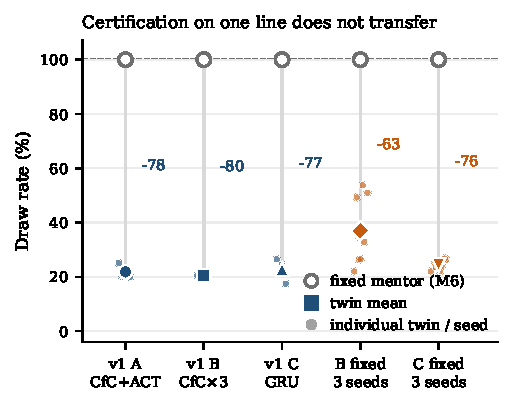
\includegraphics[width=0.96\columnwidth]{figs_v2/fig1_gap.pdf}
\caption{Twin-mentor gap. Open circles are the draw rate against the deterministic M6; filled markers are individual twins; the vertical bar is the twin mean. The v1 checkpoints and the fresh fixed-trained groups all sit at 100\% against M6 and far below it against equally strong twins.}
\label{fig:gap}
\end{figure}

\subsection{The gap is not a strength effect}
\label{sec:exact}
A natural objection is that the twins are somehow stronger than M6, or that depth 6 is a flawed teacher. Both are ruled out by the exact control in \Cref{tab:main}. The exact twins use a depth-9 solver, zero exploration, and sample uniformly among moves that are exactly optimal at depth 9. Their game-theoretic value is identical to the exact-first teacher's; they differ only in which optimal move they choose.

The exact-first teacher gives 100.0\% draws and 0.000 regret for all nine checkpoints. The exact twins give a median draw rate of 24.9\% (range 20.5--50.7), a median gap of $-75.1$ points, and regret 0.123--0.208. The exact control therefore reproduces the gap while holding teacher strength fixed. The fixed depth-6 teacher is also not making tactical errors on the lines that matter: on all 2{,}097 reachable teacher-turn boards, its depth-6 optimal action set coincides with the depth-9 exact optimal action set, and its first-choice action is exactly optimal on all of them. The failure is caused by tie-breaking, not by a weak or inexact teacher.

The weak opponent used in the original study is beaten 98--100\% of the time, and true uniform-random play is beaten 53--72\% of the time. The agents have not lost basic competence. They have lost the ability to play equally optimal lines that they did not see in training.

\subsection{How large is the tie class?}
The mechanism is visible in the state space. We enumerate every reachable board on which the agent is to move: 2{,}423 states. At each state we compute the exact depth-9 minimax value of every legal action. In 1{,}177 states (48.6\%) at least two actions are exactly optimal; the mean number of optimal actions is 1.95, and the empty board has nine. A random tie-break differs from the fixed choice on 62.3\% of the tied boards and on 30.3\% of all agent-turn boards.

The teacher's side is similar. There are 2{,}097 reachable teacher-turn boards; 937 (44.7\%) have more than one exactly optimal action, the mean optimal-set size is 1.98, and a random tie-break differs from the fixed choice on 28.6\% of teacher decisions. The teachers are equivalent in value but different in distribution. Half of the agent's decisions admit an equally optimal alternative, and a deterministic teacher collapses every such class to one action.

\section{Mechanism: The State Is the History}
\label{sec:mechanism}

\subsection{Boards versus histories}
A recurrent policy does not see the board; it sees the board plus a hidden state that is a function of the ordered history. In a Markov game the board is a sufficient statistic, but the recurrent policy's effective state space is the set of histories. We enumerate the reachable agent-turn histories by depth-first search over legal move sequences: there are 180{,}361 unique histories, compared with 2{,}423 boards, a 74.4$\times$ blow-up. Of these histories, 25{,}505 (14.1\%) end on a tied board.

The blow-up is not a technicality. The same board can be reached by different move orders, and the recurrent network can map those histories to different hidden states and different actions. A twin that breaks ties differently reaches many of the same boards by different paths. The policy may be optimal on the fixed teacher's path and wrong on the twin's path even when both paths end on the same board. This is exactly what the decision-level regret shows.

\subsection{Certification visits one line, not a state space}
The certification protocol is even smaller than the board space suggests. Against the deterministic M6, 400 games visit 5 unique boards and 5 unique histories: one line, repeated 400 times. Against 30 twins (3{,}000 games), the union is 12 unique boards and 13 unique histories. Coverage is 5/180{,}361 $=0.0028\%$ of histories for the M6 certification, and 13/180{,}361 $=0.0072\%$ for the twin ensemble. In board terms it is 0.21\% and 0.50\%. \Cref{fig:state}(a) shows the scale.

This is why a 100\% draw rate against M6 can coexist with a 24\% draw rate against twins. The certification measures one history, not the game. It also explains why the original study's 200/200 result looked like mastery: the 200 games were one deterministic line, so the effective sample size was one.

\begin{figure*}[t]
\centering
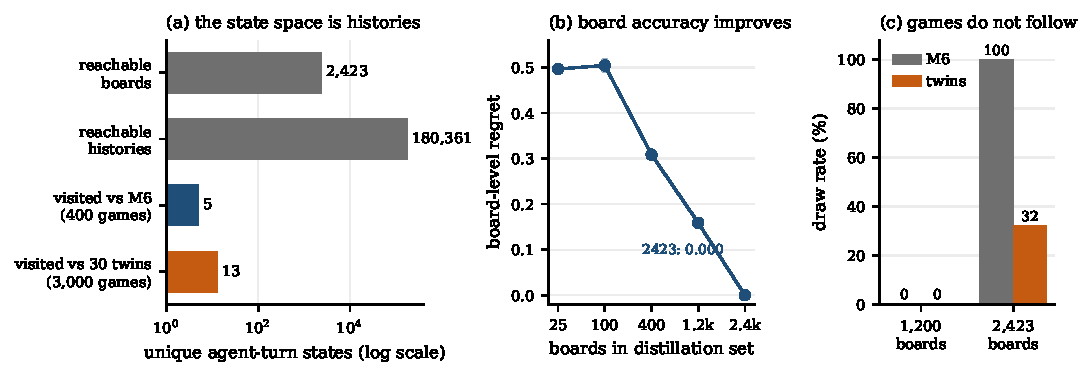
\includegraphics[width=0.98\textwidth]{figs_v2/fig3_state.pdf}
\caption{(a) Unique agent-turn states: 2{,}423 boards versus 180{,}361 histories. A 400-game certification against the deterministic mentor visits 5 histories; 3{,}000 games against 30 twins visit 13. (b) Board-level distillation on nested board subsets: regret falls as coverage grows and reaches zero with all 2{,}423 boards (two seeds). (c) Game outcomes do not follow board accuracy: the 1{,}200-board model loses every game against M6 and twins; the 2{,}423-board recurrent model draws 100\% against M6 but only 32\% against twins.}
\label{fig:state}
\end{figure*}

\subsection{Two probes: board-level and history-level}
We probe the fixed C seed-42 checkpoint in two ways. First, for each of the 2{,}423 boards we feed one canonical history (the first history found by the state enumerator) through the recurrent network and compare its greedy action with the exact optimal set. This board-level probe gives 0.518 mean regret and 0.662 optimal-action rate; on tied boards it gives 0.353 regret and 0.793 optimal action, and on non-tied boards 0.674 and 0.538. A policy that had learned the board game would score near 1.00 on both. The recurrent policy does not: even with a canonical history, it is board-suboptimal on a third of the boards.

Second, we feed every one of the 180{,}361 histories through the network with its recurrent state and compute exact regret. The mean is 0.165 and the optimal-action rate is 0.896; on the 25{,}505 tied histories the mean is 0.356 and the optimal-action rate is 0.817. The average over all histories is lower than the canonical-board probe because most histories are short and easy, not because the policy is robust: on the histories it actually visits against M6, its regret is zero, and over the full history space it is 0.165. The gap between those two numbers is the coverage problem.

\subsection{Coverage dose-response and the failure of board accuracy}
We train the GRU by distillation on nested subsets of the 2{,}423 boards: 25, 100, 400, 1{,}200, and all 2{,}423 boards, two seeds each, with soft targets uniform over the exact optimal set. \Cref{fig:state}(b) shows the board-level result. Mean board regret is 0.492/0.501 at 25 boards, 0.495/0.513 at 100, 0.305/0.312 at 400, 0.160/0.158 at 1{,}200, and 0.000/0.000 at 2{,}423. Board accuracy improves smoothly with coverage and is perfect at full coverage.

Game outcomes do not follow. The 1{,}200-board model loses all 200 games against M6 and all 200 games against each twin, despite a board-level regret of 0.160. The reason is that board-level regret averages uniformly over all 2{,}423 boards, while the policy is catastrophic on the particular non-tied boards that it visits: on those decisions, its non-tie regret is 1.0. The full 2{,}423-board model is board-optimal on the canonical history and draws 100\% against M6, but it still draws only 32.2\% against twins (range 30.5--33.8), with history-level regret 0.158 (tied histories 0.281) and optimal-action rate 0.902. \Cref{fig:state}(c) summarizes the two failures.

The lesson is two-sided. Board accuracy can be high while the visited decisions are bad (the 1{,}200-board model), and board-perfect canonical accuracy can coexist with history-level failure (the full-board recurrent model). Coverage must be measured on the state representation the policy actually uses. For a recurrent policy, that is the history space, not the board space.

\section{Teacher-Side Interventions and Their Limits}
\label{sec:tbr}

\subsection{Tie-Break Randomization is a seed lottery}
Tie-Break Randomization (TBR) changes one line of the teacher. Given the set $\mathcal{A}^{\star}(s)$ of actions with maximal minimax value,
\begin{equation}
\label{eq:tbr}
a \sim \mathrm{Uniform}\left(\mathcal{A}^{\star}(s)\right),
\end{equation}
instead of $a=\min\mathcal{A}^{\star}(s)$. The teacher's value function, depth, exploration, pity schedule, and curriculum are unchanged. TBR is distributional augmentation from an oracle: it expands the support of the teacher's behavior over the optimal equivalence class without ever choosing a suboptimal action.

\Cref{tab:lottery} and \Cref{fig:lottery} report the outcome. It is not the outcome we expected. Of the six TBR training runs, only C seed~43 is robust: it draws 100\% against M6 and 100\% against all 30 held-out twins. C seed~42 is partial: 100\% against M6 but 49.8\% against the three twins (51.3\% against 30). C seed~44 is \emph{relocated}: 75.2\% against the three twins (75.6\% against 30) but 0\% against M6. B seed~42 is also relocated: 68.5\% against twins but 0\% against M6. B seeds~43 and~44 fail both: 0\% against M6 and 0\% against twins.

The paired effect is positive for C (mean $+50.6$ points in twin draw rate, all three seeds positive, sign-flip $p=0.25$) and negative for B (mean $-14.2$ points, one positive and two negative, $p=0.75$). With three seeds the test cannot reach $p<0.05$; the point is not significance but heterogeneity. TBR does not remove the failure. It moves the certification problem: a run that is robust to twins can be fragile to the fixed mentor, because the fixed mentor's line is now the one it did not see. A single-distribution certification can be earned by any training distribution; it does not imply robustness to another.

\begin{table*}[t]
\centering
\caption{Draw rates (\%) for every training condition. ``3 twins'' uses seeds 1234/5678/9012; ``30 twins'' uses seeds 1000--1029 with 100 games each. Status: robust = 100\% against M6 and twins; partial = certified on M6 but not twins; relocated = high twin draw but fails M6; fail = fails both; none = no effect. The MLP is memoryless and has no recurrent state.}
\label{tab:lottery}
\setlength{\tabcolsep}{3pt}
\small
\begin{tabular*}{\textwidth}{@{\extracolsep{\fill}}lcccc@{}}
\toprule
\textbf{Run} & \textbf{M6} & \textbf{3 twins} & \textbf{30 twins [range]} & \textbf{Status} \\
\midrule
B fixed 42 & 100.0 & 24.9 & --- & reference \\
B TBR 42 & 0.0 & 68.5 & --- & relocated \\
B TBR 43 & 0.0 & 0.0 & --- & fail \\
B TBR 44 & 0.0 & 0.0 & --- & fail \\
C fixed 42 & 100.0 & 23.9 & 25.6 [17,36] & reference \\
C TBR 42 & 100.0 & 49.8 & 51.3 [38,59] & partial \\
C TBR 43 & 100.0 & 100.0 & 100.0 [100,100] & robust \\
C TBR 44 & 0.0 & 75.2 & 75.6 [70,84] & relocated \\
C mixed 42 & 100.0 & 43.9 & 45.3 [37,58] & partial \\
C mixed 43 & 0.0 & 0.0 & --- & fail \\
C mixed 44 & 100.0 & 50.0 & --- & partial \\
C noise 42 & 100.0 & 23.9 & --- & none \\
C noise 43 & 100.0 & 24.0 & --- & none \\
C episode 42 & 0.0 & 49.8 & --- & relocated \\
C episode 43 & 100.0 & 50.2 & 48.4 [41,55] & partial \\
C episode 44 & 0.0 & 50.0 & --- & relocated \\
MLP 0/1 & 100.0 & 100.0 & 100.0 [100,100] & robust \\
\bottomrule
\end{tabular*}
\end{table*}

\begin{figure*}[t]
\centering
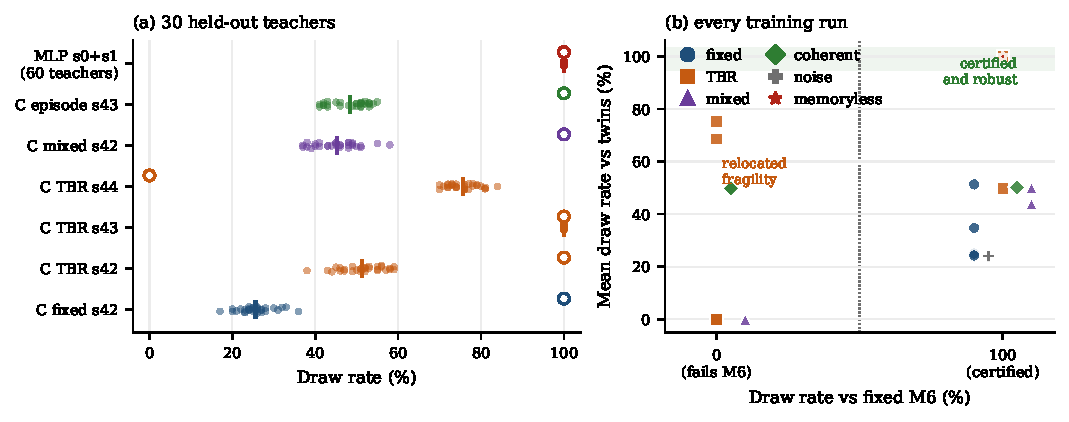
\includegraphics[width=0.98\textwidth]{figs_v2/fig2_lottery.pdf}
\caption{(a) Draw rate against 30 held-out twins for the C-backbone conditions and the memoryless MLP; the white circle marks the fixed-M6 draw rate, and the red row is the MLP. (b) Every training run in the M6/twin plane. Fixed runs (blue) are certified on M6 but fail twins. TBR runs (orange) include one robust, one partial, two relocated, and two failed runs. Mixed and coherent teachers cap near 50\%, and added noise does nothing. Only the memoryless MLP reaches the top-right corner.}
\label{fig:lottery}
\end{figure*}

\subsection{Mixed, coherent, and noisy teachers}
Three other teacher-side designs test whether more randomness helps. A \emph{mixed} teacher returns the fixed first optimal action with probability 0.5 and a random optimal action otherwise. C seeds 42--44 give 43.9\%, 0.0\%, and 50.0\% against the three twins, with 100\%, 0\%, and 100\% against M6: a lottery again. The 30-teacher mean for seed~42 is 45.3\% (range 37--58). A \emph{coherent} teacher samples one priority order over cells per game and follows it at every tied decision; C seeds 42--44 give 49.8\%, 50.2\%, and 50.0\% against twins, with 0\%, 100\%, and 0\% against M6. The 30-teacher mean for seed~43 is 48.4\% (range 41--55). Coherence stabilizes the twin rate near 50\% but does not lift it to 100\%, and it does not fix M6.

A \emph{noise} control raises the fixed mentor's exploration from 5\% to 20\%, so the teacher is more stochastic but sometimes suboptimal. C seeds 42 and 43 give 23.9\% and 24.0\% against twins, essentially the fixed baseline (23.9\% and 25.0\%); the noise does not close the gap. The distinction is practical: a noisier teacher teaches the learner to handle mistakes, but it does not systematically cover the optimal tie-break class. Only sampling within the optimal class does that, and even that is insufficient without the right learner state.

\subsection{The memoryless fix}
The constructive result is a change of state representation. We train a two-hidden-layer MLP (9--256--256--9) on the 2{,}423 reachable boards with a soft target that is uniform over the exact optimal actions at each board. Training uses 1{,}500 epochs, Adam at $10^{-3}$, two seeds. The policy is memoryless: its action depends only on the board. It is board-optimal on all 2{,}423 boards for both seeds, draws 400/400 games against M6, and draws 100\% against 60 held-out teachers: 30 random tie-breaks and 30 coherent tie-breaks, 100 games each, for each seed. It wins 97.75\% and 95.75\% against uniform random (no losses), wins 100\% against the weak minimax opponent, and has zero exact regret across 2{,}000 decisions. It is the only condition in \Cref{tab:lottery} that is certified on M6 and robust to every held-out teacher without relying on teacher-side randomization; C TBR~43 is also robust, but it is one draw from a six-run lottery.

The comparison is controlled for data, not just for architecture. The MLP sees 2{,}423 boards. A recurrent GRU distilled on the same 2{,}423 boards, but on one canonical history per board, also sees 2{,}423 training examples and is board-optimal on those canonical histories; it draws 100\% against M6. Yet over the full history space it has 0.158 regret (0.281 on tied histories, optimal-action rate 0.902), and against the three twins it draws only 32.2\% (30.5--33.8). The recurrent net memorizes the canonical path; the same board reached by a twin's different move order produces a different hidden state and a different, sometimes wrong action. The difference between 32.2\% and 100\% is not the number of boards or examples. It is the state.

\subsection{What this does and does not establish}
The MLP is a diagnostic, not an RL result: it is trained with supervised oracle labels, and it has access to the full board space. It shows that the board space is sufficient and that a memoryless policy can be robust to all tie-breaks. It does not show that an RL agent with the same budget will find such a policy. The RL agents' failure is a coverage failure induced by their recurrent state; the MLP removes the state, and with it the coverage requirement.

TBR, by contrast, requires the set of exactly optimal actions, which is available for solved games with an exact solver but not for general environments. In large games exact ties are rare and approximate ties must be defined by a tolerance; the tolerance is a new hyperparameter. TBR also increases the variance of the teacher's behavior, which can slow convergence when the optimal class is large. We observed no reliable draw-rate benefit against M6; in B it destroyed the M6 certification entirely.

\section{Worst-Case Certification over All Optimal Teachers}
\label{sec:worst}

Each comparison so far is a sample from a set. The fixed mentor is one optimal teacher, a twin is another, and the 30-teacher ensemble is thirty draws. Sampling estimates the middle of a distribution; it does not bound the extremes. In a solved game the entire set can be searched, so we replace the sample with a certificate.

\subsection{The optimal-teacher set}
Let $s$ be a board at a teacher turn and $\mathcal{A}^{\star}(s)$ the set of actions with maximal exact minimax value. A deterministic teacher is a map $\tau$ that assigns to every history $h$ ending at a teacher turn an action $\tau(h)\in\mathcal{A}^{\star}(s(h))$. Let $\mathcal{T}^{\star}$ be the set of all such maps. Every $\tau\in\mathcal{T}^{\star}$ is exactly as strong as every other: it never plays a suboptimal action, uses the same value function, and differs only in how it breaks exact ties. The fixed mentor is one element of $\mathcal{T}^{\star}$, a uniform twin is a distribution over $\mathcal{T}^{\star}$, and the 30-twin ensemble samples thirty elements.

Evaluation is deterministic, so each $\tau$ produces exactly one game against a deterministic learner $\pi$. Let $D(\tau)=1$ if that game is a draw and $0$ if the learner loses. Since $\tau$ is optimal and the learner moves first from a drawn position, the learner cannot force a win, so $D$ is binary. Define
\begin{equation}
\label{eq:cert}
\begin{aligned}
W(\pi)&=\min_{\tau\in\mathcal{T}^{\star}}D(\tau), \qquad
B(\pi)=\max_{\tau\in\mathcal{T}^{\star}}D(\tau),\\
\bar D(\pi)&=\mathbb{E}_{\tau\sim\mathrm{Unif}(\mathcal{T}^{\star})}[D(\tau)].
\end{aligned}
\end{equation}
$W$ is the worst-case draw rate, $B$ the best case, and $\bar D$ the exact average that a twin ensemble estimates. A learner is \emph{certified} if $W=1$.

\begin{proposition}[Exact certificate]
\label{prop:cert}
For a deterministic learner $\pi$, $D(\tau)\in\{0,1\}$ for every $\tau\in\mathcal{T}^{\star}$, so $W\le\bar D\le B$ and
\begin{equation}
W(\pi)=1 \iff \bar D(\pi)=1,
\end{equation}
that is, the learner draws against every $\tau\in\mathcal{T}^{\star}$.
Moreover $W$, $B$, and $\bar D$ are computable exactly by backward induction on $(\text{board},\text{history})$: a learner node has one successor, a teacher node branches over $\mathcal{A}^{\star}(s)$, and a terminal node returns $D$.
\end{proposition}

\begin{proof}
Because the learner is deterministic and the teacher is optimal, each $\tau$ yields a single draw-or-loss game, so $D(\tau)\in\{0,1\}$; an average of binary values equals one iff every value equals one, which gives the equivalence and the ordering. For the recursion, let $V_W(s,h)$ be the worst outcome from state $(s,h)$ under $\pi$. At a learner node $V_W(s,h)=V_W(s',h\cup\{s\})$, where $s'$ is the unique successor under $\pi(s,h)$; at a teacher node $V_W(s,h)=\min_{a\in\mathcal{A}^{\star}(s)}V_W(s',h)$, because the teacher may choose any optimal action at that history; terminal nodes return the game result. The recursion terminates because every move removes one empty cell. $V_B$ replaces the minimum with a maximum, and $\bar D$ with a uniform average over the teacher's branches at each node; $W$ and $B$ are attained by some $\tau\in\mathcal{T}^{\star}$ restricted to the histories reachable under $\pi$.
\end{proof}

The teacher in the recursion may choose a different tie-break at the same board reached by a different history. This is not a stronger teacher: every move it makes is still exactly optimal. It is the strongest tie-breaker inside the same strength class, which is the correct adversary for a worst-case certificate.

\subsection{Result: every fixed checkpoint has worst case zero}
We computed the certificate for all 21 recurrent checkpoints and both MLPs. \Cref{tab:certificate} reports the fixed-trained checkpoints, two informative TBR endpoints, the full-coverage recurrent distillation, and the memoryless MLP; \Cref{fig:certificate}a shows the intervals.

The first block is unanimous. For all nine fixed-trained checkpoints, $W=0$ and $B=1$: for each checkpoint there is an exactly optimal teacher that beats it, and another exactly optimal teacher that draws every game. The 100\% draw rate against the fixed mentor and the 100\% draw rate against the exact-first teacher are the best case, not a property of the checkpoint. The exact control of Section~\ref{sec:exact} removed the depth confound but not the tie-break confound, because it kept tie-breaking fixed; it is one endpoint of the interval, not its middle.

The sampled twin rate is the middle. The nine checkpoints draw 20.5--50.7\% against three exact twins, and the exact average is 25.0\% for seven of them, 37.5\% for B-43, and 50.0\% for B-44. The worst case is not 25\%; it is zero in every row. Sampling the middle says nothing about either endpoint. As a consistency check on the recursion, an independent 20{,}000-game simulation returns 25.25\% (B-v1) and 25.18\% (C-42), within Monte Carlo error of the exact 25.00\%.

The certificate is not vacuous. C-TBR-43 has $W=B=1$, as do both MLPs; the same recursion that proves the fixed checkpoints fail proves these policies robust against every optimal teacher. Across the six TBR runs, one is robust, three are mixed ($W=0$, $B=1$: B-42, C-42, C-44), and two are broken ($W=B=0$: B-43, B-44). Across the mixed, episode-coherent, and noise arms every certified run is mixed: the exact averages are 43.8\% (C-mixed-42), 43.8\% (B-episode-42), 50.0\% (C-episode-42/43), and 25.0\% (C-noise-42), all with $W=0$. The full-coverage recurrent distillation is mixed as well (33.3\%, $W=0$).

\begin{table*}[t]
\centering
\caption{Exact worst-case certification over all optimal teachers. ``M6'' and ``3 exact twins'' are sampled draw rates (\%) from the evaluations above. ``Exact mean'' is $\bar D$, the uniform average over all deterministic optimal teachers. $W$ and $B$ are the worst and best case; a run is certified only if $W=100$. ``States'' is the number of memoized $(\text{board},\text{history})$ states visited by the exact recursion.}
\label{tab:certificate}
\setlength{\tabcolsep}{4pt}
\small
\begin{tabular*}{\textwidth}{@{\extracolsep{\fill}}lrrrrrr@{}}
\toprule
\textbf{Run} & \textbf{M6} & \textbf{3 exact twins} & \textbf{Exact mean} & $\boldsymbol{W}$ & $\boldsymbol{B}$ & \textbf{States} \\
\midrule
A-v1 & 100.0 & 21.8 & 25.0 & 0 & 1 & 29 \\
B-v1 & 100.0 & 20.5 & 25.0 & 0 & 1 & 29 \\
C-v1 & 100.0 & 22.8 & 25.0 & 0 & 1 & 31 \\
B-42 & 100.0 & 24.9 & 25.0 & 0 & 1 & 30 \\
B-43 & 100.0 & 37.2 & 37.5 & 0 & 1 & 74 \\
B-44 & 100.0 & 50.7 & 50.0 & 0 & 1 & 32 \\
C-42 & 100.0 & 23.9 & 25.0 & 0 & 1 & 31 \\
C-43 & 100.0 & 26.5 & 25.0 & 0 & 1 & 27 \\
C-44 & 100.0 & 26.5 & 25.0 & 0 & 1 & 27 \\
\midrule
C-TBR-43 & 100.0 & 100.0 & 100.0 & 1 & 1 & 34 \\
C-TBR-44 & 0.0 & 75.2 & 75.0 & 0 & 1 & 34 \\
\midrule
C-distill-full & 100.0 & 32.2 & 33.3 & 0 & 1 & 38 \\
MLP (both seeds) & 100.0 & 100.0 & 100.0 & 1 & 1 & 48 \\
\bottomrule
\end{tabular*}
\end{table*}

\subsection{The exploit is three moves deep}
The certificate also returns a witness: the line that attains $W$. For C-42 the minimizing teacher wins in six plies (\Cref{fig:certificate}b):
\begin{center}
\text{O4}, \text{X2}, \text{O3}, \text{X5}, \text{O0}, \text{X8}.
\end{center}
The first four moves are optimal for both players. The agent's fifth move, O0, is its first and only suboptimal decision of the line: its exact regret is 1, and X8 completes the right column. The exploit is not a long adversarial sequence or a deeper search. It is three agent moves long, and every teacher move is exactly as optimal as the fixed mentor's.

\begin{figure*}[t]
\centering
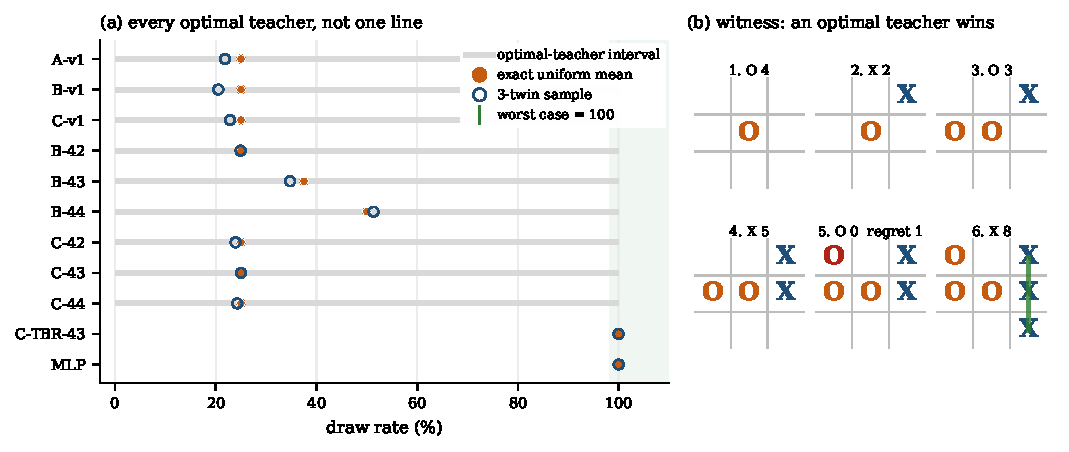
\includegraphics[width=0.98\textwidth]{figs_v2/fig5_certificate.pdf}
\caption{(a) The optimal-teacher interval $[W,B]$ for the fixed checkpoints, C-TBR-43, and the memoryless MLP. The gray bar is the full interval; the orange dot is the exact uniform mean $\bar D$; the blue circle is the three exact-twin sample; a green tick marks $W=100$. Every fixed checkpoint has the interval $[0,100]$: the same policy is helpless against one optimal teacher and perfect against another. (b) The six-ply witness for C-42. The first four moves are optimal for both players; O0 (red) is the agent's only suboptimal decision, with exact regret 1, and X8 completes the right column (green).}
\label{fig:certificate}
\end{figure*}

\subsection{Board optimality certifies; canonical board optimality does not}
\begin{proposition}[Board-optimal policies are worst-case robust]
\label{prop:board}
If a deterministic learner is board-optimal at every reachable agent-turn board, then $W(\pi)=1$ against every deterministic optimal teacher.
\end{proposition}

\begin{proof}
If both players choose a value-maximizing action at every decision, the game follows an optimal line from a drawn initial position. By backward induction on the game tree, the value of every visited state is zero from the learner's perspective, so the game is a draw for every $\tau\in\mathcal{T}^{\star}$.
\end{proof}

The converse fails for recurrent policies. The full-coverage GRU is board-optimal on all 2{,}423 canonical histories---it is the distillation that draws 100\% against M6---and over the full history space it has 0.158 regret. Its certificate is $W=0$: some optimal teacher beats it. Board-optimality on one history per board is an average-case property; it does not imply board-optimality on the histories that the game actually visits, and it does not imply a worst-case guarantee. The memoryless MLP, whose action depends only on the board, satisfies the premise of \Cref{prop:board} and has $W=B=1$.

This is the cleanest statement of the representation result. The difference between the MLP and the recurrent distillation is not data or teacher strength; the next subsection adds direct controls showing that it is not parameter count either. It is whether the policy's state is the board or the history. A board state makes $W=1$ attainable; a history state makes the same board a different decision problem on every move order.

\subsection{Is it model size?}
\label{sec:size}
A reviewer may object that the failing networks are simply too small: a larger model would learn the tie classes and the gap would close. Four controls, all with exact certificates, say otherwise. They separate parameter count from the two variables that actually matter, the teacher's tie policy and the policy's state.

\emph{Size is neither necessary nor sufficient.} The certified memoryless MLP has 70{,}665 parameters, 4.6 times fewer than the 323{,}491-parameter GRU that fails. The certified C-TBR-43 has the same architecture, the same parameter count, and the same 5{,}000-game curriculum as C-42; only the mentor's tie-break differs, and that takes the certificate from $W=0$ to $W=B=1$ (one run in six; TBR is a seed lottery, so this is an existence proof at fixed size, not a reliable recipe).

\emph{Widening the failing model does not help.} We retrained the GRU with 600 hidden units (1{,}185{,}691 parameters, 3.7 times the original) on the same 2{,}423 canonical histories, with the same exact depth-9 soft targets and 400 epochs. Both widths fit the training set perfectly (zero regret and optimal-action rate 1.00 on all 2{,}423 states; soft cross-entropy 0.551 versus 0.546), so the comparison is not confounded by underfitting. Over all 180{,}361 histories the wide model has mean regret 0.155--0.157 and optimal-action rate 0.903, against 0.158 and 0.902 for the original; its certificate is still $W=0$, $B=1$ for both seeds. A 3.7-fold increase in parameters changes average regret by at most 0.003 and does not remove the worst case.

\emph{Average regret is not the certificate.} Complete history coverage at the original size does move the average: training the same GRU on all 180{,}361 histories with exact optimal-set targets reduces mean history regret from 0.158 to 0.005 (30-fold) and raises the optimal-action rate to 99.6\%, yet the certificate is still $W=0$, $B=1$. Conversely, C-TBR-43 has a \emph{higher} mean history regret (0.185) than C-42 (0.165) and is certified. The reason is that the certificate visits only states reachable under optimal play: C-TBR-43's residual errors lie off that tree, whereas the full-history GRU's residual 0.4\% lies on it, and a single losing line is enough to make $W=0$. Average accuracy over an enormous history space is therefore neither necessary nor sufficient for robustness on the tree that decides the game.

\emph{What does predict robustness.} The two certified policies differ either in teacher (randomized ties at fixed size) or in state (board instead of history, at 4.6 times fewer parameters). The two fragile recurrent policies share a history state and a deterministic teacher. Parameter count does not separate the rows of \Cref{tab:size}; the teacher's tie policy and the policy's state do.

\begin{table*}[t]
\centering
\caption{Model-size controls. Mean history regret is exact minimax regret over all 180{,}361 agent-turn histories; it differs from the game-level $r_{\text{twin}}$ of \Cref{tab:main}, which averages only over decisions reached in play. The exact mean is the uniform average draw rate over all optimal teachers, and $W,B$ are its minimum and maximum. The first two rows share architecture, width, and the 5{,}000-game curriculum; only the mentor's tie-break differs. The 600-wide run repeats the 300-wide board-level distillation at double width; the full-history run repeats it with all 180{,}361 histories instead of 2{,}423. Both use the same exact depth-9 soft targets and a deterministic teacher. The MLP is memoryless.}
\label{tab:size}
\small
\begin{tabular*}{\textwidth}{@{\extracolsep{\fill}}lrlcccc@{}}
\toprule
\textbf{Model} & \textbf{Params} & \textbf{Training} & \textbf{History regret} & \textbf{Exact mean} & $W$ & $B$ \\
\midrule
C-42 (GRU 300) & 323{,}491 & RL, 5k, fixed ties & 0.165 & 25.0 & 0 & 1 \\
C-TBR-43 (GRU 300) & 323{,}491 & RL, 5k, random ties & 0.185 & 100.0 & 1 & 1 \\
GRU 600, s0/s1 & 1{,}185{,}691 & distillation, 2{,}423 boards & 0.155/0.157 & 68.8/50.0 & 0 & 1 \\
GRU 300, full history & 323{,}491 & distillation, 180{,}361 histories & 0.005 & 37.5 & 0 & 1 \\
MLP 256 & 70{,}665 & distillation, 2{,}423 boards & 0.000 & 100.0 & 1 & 1 \\
\bottomrule
\end{tabular*}
\end{table*}

\subsection{Cost and scope}
The exact recursion is small. It visits 27--90 memoized $(\text{board},\text{history})$ states per recurrent checkpoint and 48 for the MLP, because the learner's deterministic policy selects one action per history and only the teacher's tie-breaks create width. The expensive step is evaluating the policy once on all 180{,}361 histories (about 24 seconds on one CPU core); the certificate itself is negligible. For comparison, a 400-game certification visits 5 boards and 5 histories, and the 30-twin suite visits 12 boards and 13 histories.

The certificate requires an exact solver and a deterministic learner, both available here. For approximate ties, $\mathcal{A}^{\star}$ becomes the set of actions within a tolerance $\epsilon$ of the maximum; the certificate is then relative to that tolerance, which must be reported. For large games the recursion remains exact in principle, but its state count is the number of states reachable under the learner against all optimal teachers, which can grow quickly; a sampled lower bound on $W$ is then the practical fallback, and it should be reported as a lower bound, not as a certificate.

\section{From Certificate to Repair}
\label{sec:repair}

The certificate answers a yes/no question. It also returns the states that decide the answer. This section uses that by-product as a training signal: the same backward induction that proves a policy fragile identifies the histories on which it must be corrected, and correcting only those histories is sufficient.

\subsection{The frontier}
For a deterministic learner $\pi$, let $R(\pi)$ be the set of learner-turn histories reachable when the teacher plays an action from $\mathcal{A}^{\star}(s)$ at every teacher turn and the learner follows $\pi$. This is exactly the set traversed by the recursion of \Cref{prop:cert}. It is policy-dependent, and it is small: for the checkpoints in this paper $|R(\pi)|$ ranges from 4 to 19, against 5{,}097 agent histories in the optimal-play tree (both players optimal) and 180{,}361 in the full history space.

\begin{lemma}[Frontier sufficiency]
\label{lem:frontier}
If $\pi$ plays an optimal action at every state in $R(\pi)$, then $W(\pi)=1$.
\end{lemma}

\begin{proof}
Assume $\pi(h)\in\mathcal{A}^{\star}(s(h))$ for every $h\in R(\pi)$. The root of the restricted tree is the empty board, whose minimax value is zero. At a learner node the chosen action is optimal, so the node and its unique successor have the same value; at a teacher node every action in $\mathcal{A}^{\star}$ preserves the value. By backward induction, every node in the restricted tree therefore has value zero, so every terminal node is a draw. Hence $D(\tau)=1$ for every $\tau\in\mathcal{T}^{\star}$.
\end{proof}

The lemma is the constructive counterpart of \Cref{prop:board}: board-optimality is sufficient because it implies optimality on every history, but it is not necessary. Optimality on the frontier is necessary and sufficient, and the frontier is typically two orders of magnitude smaller than the history space. The difficulty is that $R(\pi)$ depends on $\pi$: changing the policy changes the tree that must be repaired.

In practice the oracle is often approximate. The same argument survives with a tolerance, and it is worth stating because it fixes what an approximate certificate can and cannot promise. Let the oracle be $\varepsilon$-accurate, $|\tilde Q(s,a)-Q^{\star}(s,a)|\le\varepsilon$, and let $B_\varepsilon(s)=\{a:Q^{\star}(s,a)\le V^{\star}(s)+\varepsilon\}$ be the near-optimal teacher actions. Write $R_\varepsilon(\pi)$ for the frontier reached when the teacher plays in $B_\varepsilon$ and the learner follows $\pi$.

\begin{proposition}[Approximate certificates]
\label{prop:approx}
Let outcomes lie in $\{-1,0,1\}$, let $V^{\star}(\emptyset)=0$, and let $H$ be the horizon. If $\pi$ maximizes the estimated $Q$ at every state of $R_\varepsilon(\pi)$ and $2\varepsilon H<1$, then $\pi$ does not lose against any teacher that plays in $B_\varepsilon$ at every turn.
\end{proposition}

\begin{proof}
At a learner node $s$ with successors $s'$, choosing the estimated maximizer gives $Q^{\star}(s,\pi(s))\ge V^{\star}(s)-2\varepsilon$, so $D(s)=V^{\pi,\tau}(s)-V^{\star}(s)\ge D(s')-2\varepsilon$. At a teacher node the teacher's action satisfies $V^{\star}(s')\ge V^{\star}(s)$, so $D(s)\ge D(s')$ and the node adds nothing. Along any path there are at most $H$ learner nodes and $D=0$ at the terminal, hence $D(\emptyset)\ge-2\varepsilon H>-1$. Terminal payoffs and $V^{\star}(\emptyset)$ are integers, so $D(\emptyset)\ge0$: the learner draws or wins.
\end{proof}

The proposition is the tolerance version of \Cref{lem:frontier}, and its cost scales with the number of learner moves rather than the horizon. It also says what changes with an approximate oracle: the certified teacher class grows from the exactly optimal actions to the $\varepsilon$-optimal ones, and the guarantee degrades from no loss to a loss of at most $2\varepsilon H$. The tolerance must therefore be reported as a fraction of $1/H$, not as an absolute number. All experiments in this paper use exact oracles, so $\varepsilon=0$ and the proposition reduces to the lemma; the Rock-Paper-Scissors certificate is exact for its Bayesian objective in the same way.

\subsection{Certificate-guided repair}
\Cref{alg:cgr} closes the loop. Each round certifies the current policy, stops if $W=1$, and otherwise adds the violating frontier histories---with targets uniform over the exact optimal set---to an aggregate that is fitted together with a replay set. The model, its width, and the teacher are unchanged; only the histories seen by the optimizer change.

\begin{algorithm}[t]
\caption{Certificate-Guided Repair (CGR)}
\label{alg:cgr}
\begin{algorithmic}[1]
\REQUIRE policy $\pi$, replay set $\mathcal{D}_0$, exact oracle $V$, optimal-teacher set $\mathcal{T}^{\star}$
\STATE $\mathcal{A}\gets\emptyset$
\FOR{round $=1,2,\dots$}
  \STATE compute $W(\pi)$, $B(\pi)$, $\bar D(\pi)$, and $R(\pi)$ by backward induction
  \IF{$W(\pi)=1$}
    \RETURN $\pi$ \COMMENT{certified against every $\tau\in\mathcal{T}^{\star}$}
  \ENDIF
  \STATE $\mathcal{A}\gets\mathcal{A}\cup\{h\in R(\pi):\pi(h)\notin\mathcal{A}^{\star}(s(h))\}$
  \STATE fine-tune $\pi$ on $\mathcal{D}_0\cup\mathcal{A}$ with targets uniform over $\mathcal{A}^{\star}$, until $\mathcal{A}$ fits
\ENDFOR
\end{algorithmic}
\end{algorithm}

\begin{proposition}[Soundness and progress]
\label{prop:cgr}
Every policy returned by \Cref{alg:cgr} is certified exactly: $W=1$ against every deterministic optimal teacher, not only against the sampled twins. If the fit step reaches zero regret on $\mathcal{A}$, then every non-terminal round adds at least one new history to $\mathcal{A}$, so the loop terminates after at most $H$ rounds, where $H$ is the number of agent-turn histories.
\end{proposition}

\begin{proof}
The stopping test is the exact recursion of \Cref{prop:cert}, so a returned policy has $W=1$. If the aggregate is fitted exactly and $W=0$, \Cref{lem:frontier} implies that some $h\in R(\pi)$ is not optimal, and that $h$ is not in $\mathcal{A}$ (all states in $\mathcal{A}$ have zero regret); hence the round adds a new history. The aggregate is a subset of a finite set, so the loop cannot add new histories forever.
\end{proof}

In practice we also cap the number of rounds and the epochs per round; if a fit does not reach zero aggregate regret, the certificate still governs the final answer, but the progress argument does not apply. In every repair round reported below the aggregate was fitted to zero regret, within eight epochs. The 2{,}423-history canonical set is used as replay, and the aggregate is oversampled 60 times so that a handful of histories is not diluted; no other hyperparameter changes.

\subsection{Repairing the failing checkpoints}
\Cref{tab:repair} applies CGR to three policies that the certificate rejects. The first is the RL checkpoint C-42 of \Cref{tab:main}: 323{,}491 parameters, five thousand games against the fixed mentor, $W=0$, $\bar D=25.0\%$. Four rounds and seven histories take it to $W=B=1$ and $\bar D=100\%$. The seven histories are distinct boards; the frontier at the last round has no violations. The independent implementation of \texttt{worst\_case\_eval.py} re-certifies the saved checkpoint at $W=B=1$ over 26 states, so the result does not depend on the repair script's own recursion.

The second is the GRU distilled on all 180{,}361 histories (Section~\ref{sec:size}). Its mean history regret is 0.005 and its exact average is 37.5\%, yet $W=0$: the residual errors that matter lie on the optimal-play tree. Two rounds and five histories take it to $W=B=1$, and the all-history regret moves from 0.00526 to 0.00538, within noise of the original. This is the sharpest statement of the paper's thesis: complete history coverage did not remove the worst case, and five selected histories did.

The third is a GRU distilled for only 20 epochs, which is broken in the strong sense: $W=B=0$, $\bar D=0$. Two rounds and three histories take it to $W=B=1$ and $\bar D=100\%$, with all-history regret moving from 0.0346 to 0.0388: even a policy that loses to every optimal teacher has a three-state repair.

The control is matched in rounds, states, optimizer, epochs, and fitting protocol. Controls add the same number of histories per round, sampled uniformly either from all 180{,}361 histories or from the 5{,}097-history optimal-play tree, without looking at violations. None of the eighteen controls reaches $W=1$: for C-42 all six stay at $\bar D=25.0\%$, for the full-history model the six end between 25.0\% and 50.0\% (base 37.5\%), and for the broken model all six stay at 0. Several random additions improve the average while leaving the worst case at zero; selecting the states, not adding states, is what repairs the policy.

A third arm closes the boundary. DAgger \cite{ross2011} queries the learner's own rollout distribution with exact labels, and in these games it sometimes works. In Tic-Tac-Toe the matched-budget arm adds exactly CGR's seven states and fails in all three seeds; the unconstrained arm certifies in two of three, but needs 20 states, and in the third seed it adds 72---ten times CGR's budget---and still does not certify. In Connect Three the matched arm certifies two of three seeds at 11 states, the same count CGR spends, and the unconstrained arm certifies two of three at 27--32 (Table~\ref{tab:dagger}). DAgger is therefore competitive exactly where the frontier is small enough to be hit by visitation, and its failures are not budget failures: the 72-state Tic-Tac-Toe run visits every state its policy reaches under random optimal teachers and still misses a violating history, because those teachers never take the game down the tie-break line that decides the certificate. The certificate's contribution is not that it beats on-policy sampling in every game; it is that the states it selects are the ones the test names, so the same budget certifies in every seed.

\begin{table}[t]
\centering
\caption{DAgger under the exact certificate. All arms use the same oracle, stopping test, optimizer and epochs; ``states'' is the number of added histories and ``certified'' counts seeds reaching $W=1$. The matched arms receive CGR's per-round counts; the full arms add every visited state.}
\label{tab:dagger}
\setlength{\tabcolsep}{3pt}
\footnotesize
\begin{tabular}{@{}lccc@{}}
\toprule
\textbf{Domain} & \textbf{Arm} & \textbf{States} & \textbf{Certified} \\
\midrule
Tic-Tac-Toe, C-42 & CGR & 7 & 1/1 \\
 & DAgger, matched & 7 & 0/3 \\
 & DAgger, full & 20--72 & 2/3 \\
\midrule
Connect Three & CGR & 8--11 & 3/3 \\
 & DAgger, matched & 11 & 2/3 \\
 & DAgger, full & 27--32 & 2/3 \\
\midrule
Rock-Paper-Scissors & CGR & 39--53 & 3/3 \\
 & DAgger, all types & 53 & 1/3 \\
 & DAgger, worst type & 43 & 0/3 \\
\bottomrule
\end{tabular}
\end{table}

\begin{table*}[t]
\centering
\caption{Certificate-guided repair. ``Before'' and ``After'' are the exact worst case $W$, best case $B$, and uniform optimal-teacher average $\bar D$ (\%). ``Added'' counts distinct learner histories added to the 2{,}423-history replay set; ``Rounds'' counts certificate-fit rounds. History regret is exact mean minimax regret over all 180{,}361 histories. The same model, width, and teacher are used before and after; only the training histories change.}
\label{tab:repair}
\setlength{\tabcolsep}{4pt}
\small
\begin{tabular*}{\textwidth}{@{\extracolsep{\fill}}lrlcccr@{}}
\toprule
\textbf{Target} & \textbf{Params} & \textbf{Before $W/B/\bar D$} & \textbf{Added} & \textbf{Rounds} & \textbf{After $W/B/\bar D$} & \textbf{History regret} \\
\midrule
C-42 (RL, fixed ties) & 323{,}491 & 0/1/25.0 & 7 & 4 & 1/1/100.0 & 0.165 $\to$ 0.171 \\
Full-history GRU & 323{,}491 & 0/1/37.5 & 5 & 2 & 1/1/100.0 & 0.0053 $\to$ 0.0054 \\
Broken GRU (20 epochs) & 323{,}491 & 0/0/0.0 & 3 & 2 & 1/1/100.0 & 0.035 $\to$ 0.039 \\
\bottomrule
\end{tabular*}
\end{table*}

\begin{figure*}[t]
\centering
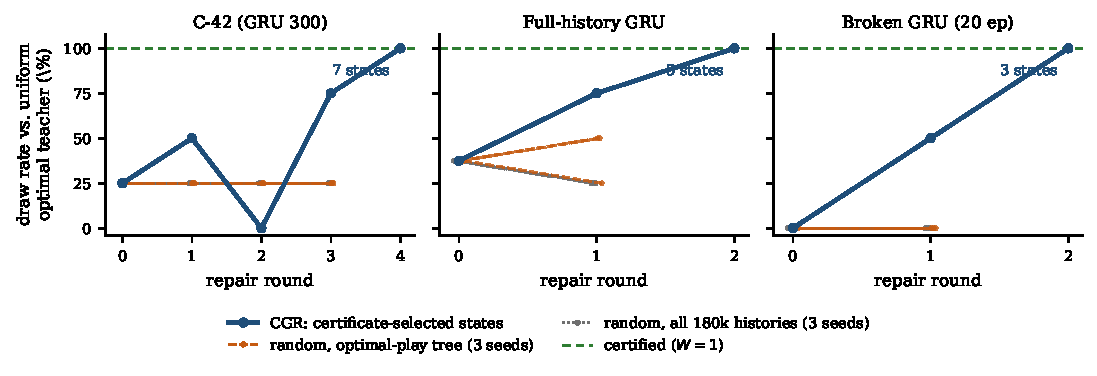
\includegraphics[width=0.92\textwidth]{figs_v2/fig6_repair.pdf}
\caption{Exact uniform optimal-teacher draw rate after each repair round for C-42 (left), the full-history GRU (middle), and the 20-epoch GRU that initially loses to every optimal teacher (right). Certificate-selected states (blue) reach 100\% in four, two, and two rounds. Matched random aggregation with the same number of states does not, whether the states are drawn from all 180{,}361 histories (dotted) or from the 5{,}097-history optimal-play tree (dashed); some random draws lower the average. Intermediate CGR policies can regress (C-42 falls to 0 after round 2); the next certificate catches the regression and the following round repairs it. The horizontal line is $W=1$.}
\label{fig:repair}
\end{figure*}

\subsection{Why selection matters}
The frontier is a policy-dependent sufficient statistic for robustness. It is not the set of histories that are hardest on average, nor a uniform sample of the optimal-play tree: it is the set that the current policy actually reaches while the teacher chooses adversarial tie-breaks, and it changes as the policy changes. A static data distribution cannot target it, which is why full-history coverage leaves a 0.4\% residual on exactly the states that decide the game, while five selected states remove it. An on-policy distribution can miss it as well: DAgger samples the states the current policy reaches against sampled optimal teachers, and those teachers do not choose the tie-break line on which the certificate fails (Table~\ref{tab:dagger}). CGR is dataset aggregation \cite{ross2011} over the optimal tie-break class, with the exact certificate supplying both the query states and the stopping test.

The price is a small loss of average accuracy off the frontier: C-42's history regret rises from 0.165 to 0.171 while its worst case goes from 0 to 1. The trade is the point of the paper---average regret over the history space is neither necessary nor sufficient for robustness---and it is the right trade when certification is the goal. The method requires an exact oracle and a deterministic learner; with approximate ties the frontier is defined relative to a tolerance, and each round still ends with a certificate relative to that tolerance. In larger games the frontier grows with the number of optimal lines, and each round costs one policy evaluation over the reachable tree; the recursion, not the training, is the binding cost.

\subsection{A second domain: Connect Three}
CGR was developed on Tic-Tac-Toe. To test whether the phenomenon and the method depend on that game, we built an exact oracle for \emph{Connect Three} on a $4\times3$ board (four rows, three columns, three in a row, gravity). The game is small enough to enumerate completely: 2{,}715 reachable boards, of which 933 are learner-turn positions. We trained a 14{,}443-parameter GRU with the same architecture on one canonical history per learner-turn board (933 items), with soft targets uniform over the exact optimal action set, and stopped only when all 933 decisions were optimal. The base policy therefore has zero board-level mistakes. Its exact certificate nevertheless gives $W=0$, $B=1$, and $\bar D=11.1\%$, $22.2\%$, $33.3\%$ for seeds 0--2, and it loses to every deterministic optimal teacher in the first two seeds ($0/6$ drawn; seed 2 draws two of six). In each seed the certificate finds four to six violating histories, and all of them are \emph{alternative histories to boards that the policy already plays optimally}. Board coverage is complete and the failure remains: the missing variable is the move order, exactly as in Tic-Tac-Toe.

CGR with the same protocol---add the violating frontier histories, oversample them $60\times$, refit the same model, and stop when both the 933-item replay and the aggregate are exactly optimal---certifies all three seeds (\Cref{tab:c4}). Eleven, nine, and eight selected histories take five, five, and two rounds to reach $W=1$. The repaired policies keep zero mistakes on all 933 board histories, so the repair adds robustness without sacrificing board accuracy. An independent memo-free recursion (\texttt{c4\_verify.py}) re-certifies each saved checkpoint at $W=1$: all six deterministic column-order teachers draw, and 2{,}000 randomly adaptive optimal teachers draw 100\%. Intermediate policies can regress on the average (seed 1 rises to 88.9\% and falls to 66.7\%) while the certificate keeps returning the violations; $W$ reaches 1 only when the frontier is empty (\Cref{fig:c4}).

The controls are matched in rounds, states, optimizer, epochs, and stopping rule. Eighteen controls add the same number of histories per round, sampled without looking at violations from constrained random-play histories or from the optimal-play tree. None certifies: all eighteen stay at $W=0$, and their averages never exceed the largest base average (33.3\%); several are identical to their base. Selection, not the number of added histories, is again what repairs. DAgger, matched in the same way, is the boundary case: it certifies two of three seeds at the same 11 states and fails the third, and with all visited states it also certifies two of three at 27--32 (Table~\ref{tab:dagger}). In this game the frontier has five states, small enough for an on-policy sampler to hit it; the Tic-Tac-Toe frontier has thirteen and matched DAgger never hits it.

\begin{table}[t]
\centering
\caption{Certificate-guided repair on Connect Three ($4\times3$). $W/B/\bar D$ are exact worst case, best case, and uniform optimal-teacher average (\%). ``Added'' counts distinct learner histories added to the 933-history board replay; ``Repl.'' is the number of board histories that are not optimal after repair.}
\label{tab:c4}
\setlength{\tabcolsep}{3pt}
\footnotesize
\begin{tabular}{@{}lcccccc@{}}
\toprule
\textbf{Seed} & \textbf{Before $W/B/\bar D$} & \textbf{Viol.} & \textbf{Added} & \textbf{Rounds} & \textbf{After $W/B/\bar D$} & \textbf{Repl.} \\
\midrule
0 & 0/1/11.1 & 6 & 11 & 5 & 1/1/100.0 & 0 \\
1 & 0/1/22.2 & 5 & 9 & 5 & 1/1/100.0 & 0 \\
2 & 0/1/33.3 & 4 & 8 & 2 & 1/1/100.0 & 0 \\
\bottomrule
\end{tabular}
\end{table}

\begin{figure*}[t]
\centering
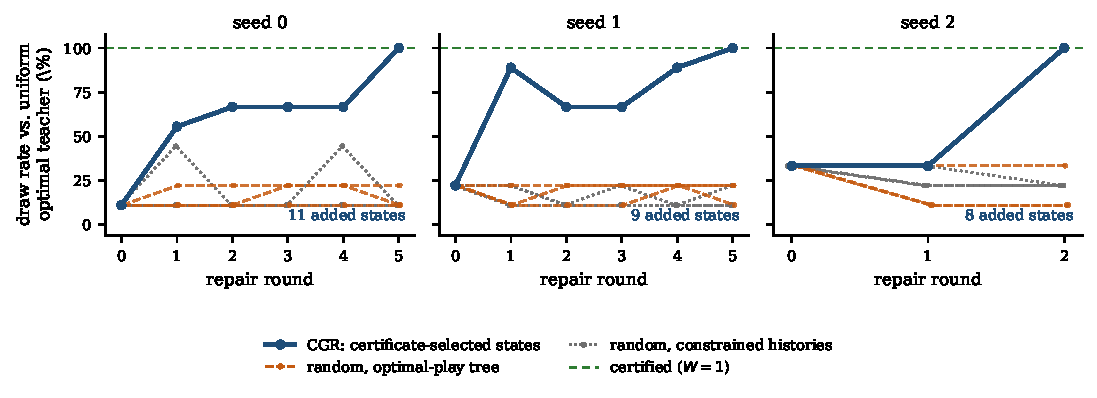
\includegraphics[width=\textwidth]{figs_v2/fig7_c4.pdf}
\caption{Connect Three ($4\times3$). Exact uniform optimal-teacher draw rate after each repair round for three seeds. Certificate-selected histories (blue) reach 100\% in five, five, and two rounds; matched random additions of the same size from the constrained-history pool (dotted) or from the optimal-play tree (dashed) never do. Intermediate CGR policies can regress on the average while still reducing the violation count; the horizontal line is $W=1$.}
\label{fig:c4}
\end{figure*}

\subsection{Connect Four on a $4\times4$ board}
The next step is a real Connect Four board ($4\times4$, four in a row), with 161{,}029 reachable positions. A canonical replay over every learner board is too large, so the base policy is trained on the 4{,}328 learner histories of the tree generated by one deterministic optimal teacher; 194 of them are constrained. It reaches zero mistakes on that tree, and the exact certificate gives $W=0$, $B=1$, $\bar D=32.8\%$: twelve of the 24 deterministic column orders draw, and the frontier contains 946 states and 75 violations. CGR with the standard stopping rule (a refit stops when the aggregate is optimal) adds 1{,}182 histories over 33 rounds and reaches $W=B=1$; the final policy also has zero replay mistakes. The certificate grows from 2{,}307 to 8{,}877 states and the frontier from 946 to 3{,}572, so certification and repair cost more, but the loop still closes. Independent verification gives $W=1$, 24/24 deterministic orders draw, and 2{,}000 adaptive optimal teachers draw 100\%.

Two matched controls add 1{,}181 histories with the same per-round budget and optimizer, sampled without looking at violations from constrained random play or from the optimal-play tree; under a ten-epoch per-round cap they use 104 and 68 optimizer epochs against 116 for the repair arm. Both remain at $W=0$ (108 and 117 violating histories): the constrained-history control raises $\bar D$ from 32.8\% to 48.2\%, while the optimal-play-tree control ends at 32.5\%, below the base. Random aggregation moves the average but not the worst case.

\subsection{Endgames on the full $7\times6$ board}
The full $7\times6$ game is not enumerable here, but endgames with eight empty cells are. We sample 40 roots by random play to eight empty cells, keep those whose exact value is a draw, and solve each root exactly; their prefixes are random histories. The three seeds share the same 40-root suite, so seed differences cannot be attributed to a different endgame sample. Each base GRU (57k parameters) is trained on its own sample of learner histories inside the roots - 498, 461 and 503 for seeds 0--2 - and is exact on all of them. The conditional certificate over all teacher tie-breaks below the roots gives $W=0$, $B=1$, and $\bar D=76.6\%$, $78.9\%$, $79.4\%$ for seeds 0--2; 22, 25, and 23 of the 40 roots are drawn on average and 43, 42, and 40 violating histories remain. CGR adds 111, 102, and 95 histories in eight, six, and seven rounds and reaches $W=B=1$ in all three seeds: every root is drawn against 120 sampled deterministic column orders and against 40 random adaptive optimal teachers per root (verified for seed 0 by a separate memo-free recursion). One, three, and one replay decision of those sets is not optimal after repair, so the exact guarantee costs a handful of board decisions. The certificate is exact conditional on the sampled suite, not for the full $7\times6$ game; within that scope, the mechanism extends to a board where exhaustive global certification is out of reach, and its round count is stable across seeds.

Six matched controls on seed~0 add histories with the same per-round budget (105--111 unique constrained histories were available) and refit with the same optimizer and stopping rule. All six stay at $W=0$, with $\bar D$ between 75.2\% and 92.1\%. The three optimal-play-tree controls reach 87.6--92.1\% on average, close to the certified policy's 100\%, yet each still contains a root where an optimal teacher wins. Matched aggregation can almost match the average; only certificate-selected histories remove the worst case.

\subsection{Going deeper: ten empty cells on the same board}
\label{sec:ten}
Depth, not board size, is the scaling axis. The same $7\times6$ board with ten empty cells keeps every root exactly solvable while lengthening the histories the certificate must traverse. As in the eight-cell arms, the three seeds read one shared 40-root suite, so the differences below are policy differences rather than sample differences; each seed draws its own base replay, which holds 1{,}038, 1{,}151 and 1{,}089 learner histories (182, 200 and 199 of them constrained) against 498, 461 and 503 at eight empty cells. Nothing about the eight-cell result breaks: all three base policies have $W=0$ and $B=1$, with $\bar D=68.2\%$, $72.9\%$ and $72.6\%$, 59, 48 and 49 violating histories, and 18, 19 and 17 of the 40 roots drawn. The violating frontier is still finite and still enumerable exactly.

What changes is the price of closing it, and how unevenly that price is paid across seeds. On seed 0 CGR reduces violations 59 $\to$ 39 $\to$ 20 $\to$ 19 $\to$ 11 $\to$ 15 $\to$ 6 $\to$ 9 $\to$ 9 $\to$ 3 $\to$ 6 $\to$ 5 $\to$ 3 $\to$ 5 $\to$ 2 $\to$ 2 $\to$ 1 $\to$ 0 and is \emph{not} certified after the ten rounds the eight-cell suite needed; 17 rounds and 214 certificate-selected histories reach $W=B=1$ with $\bar D=100\%$. Seed 1 takes 14 rounds and 166 histories (48 $\to$ 40 $\to$ 19 $\to$ 14 $\to$ 15 $\to$ 11 $\to$ 2 $\to$ 6 $\to$ 1 $\to$ 3 $\to$ 1 $\to$ 2 $\to$ 3 $\to$ 1 $\to$ 0) and seed 2 only 7 rounds and 166 (49 $\to$ 58 $\to$ 22 $\to$ 16 $\to$ 10 $\to$ 7 $\to$ 4 $\to$ 0). All three end certified and all three keep zero mistakes on their base replay, where the eight-cell arms lost one, three and one replay decision: the deeper arms are repaired on a larger aggregate, repeated 60 times, so the extra depth costs rounds without costing exactness on the training set. The spread in rounds nevertheless widens, from 6--8 at eight empty cells to 7--17 here: the median cost of eight more empty cells is roughly a doubling of rounds (7 $\to$ 14) and of added histories (102 $\to$ 166), while the certificate stays exact and the model is unchanged (57k parameters, hidden 128). At greater depth the same exact procedure has a less predictable cost, and one arm no longer characterizes it.

The refit budget is also the one place the ten-cell arms differ from the eight-cell arms---each added history is repeated 60 times instead of 20, and a refit stops only when both the replay set and the aggregate are exactly optimal, where the eight-cell arm stopped on the aggregate alone---so the extra rounds are not bought with a weaker certificate or a weaker stopping rule. The intermediate non-monotonicity is the same effect visible in Connect Three: refitting on a larger aggregate can unlearn an earlier frontier state before the next round re-adds it, which is why the stopping rule is the certificate and not the training loss. Seed 0 shows it at 11 $\to$ 15, seed 1 twice at 14 $\to$ 15 and 2 $\to$ 6, and seed 2 on its very first refit, where violations rise 49 $\to$ 58 before the trajectory falls to zero.

The two matched controls on seed 0's ten-cell suite also fail, and they fail with \emph{more} data than the eight-cell controls used. Constrained-pool aggregation with 182 added histories ends at $W=0$, $\bar D=73.0\%$, 49 violations; optimal-play-tree aggregation with 150 added histories ends at $W=0$, $\bar D=87.0\%$, 36 violations. The tree control again lands close to a certified policy on the average and still contains a root an optimal teacher wins. All three repaired checkpoints are re-certified by the separate memo-free recursion: $W=B=1$, every root drawn by all 120 sampled deterministic column orders and by 40 random adaptive optimal teachers per root, in each seed.

\begin{table}[t]
\centering
\caption{Scaling the $7\times6$ endgame suite at fixed board, model and root count (40 draw-valued roots, GRU hidden 128). ``Rounds'' counts certificate--refit rounds, ``Added'' counts distinct histories the certificate selected, and $\bar D$ is the uniform optimal-teacher draw rate (\%). ``Controls'' is the number of matched random-aggregation arms reaching $W=1$ out of those run on that seed; controls were run on seed 0 only.}
\label{tab:scaling76}
\setlength{\tabcolsep}{4pt}
\footnotesize
\begin{tabular}{@{}llrrrrc@{}}
\toprule
\textbf{Empty} & \textbf{Seed} & \textbf{Rounds} & \textbf{Added} & \textbf{$W$} & \textbf{$\bar D$} & \textbf{Controls} \\
\midrule
8  & 0 & 8 & 111 & $0\to1$ & $76.6\to100$ & 0/6 \\
8  & 1 & 6 & 102 & $0\to1$ & $78.9\to100$ & -- \\
8  & 2 & 7 & 95  & $0\to1$ & $79.4\to100$ & -- \\
\midrule
10 & 0 & 17 & 214 & $0\to1$ & $68.2\to100$ & 0/2 \\
10 & 1 & 14 & 166 & $0\to1$ & $72.9\to100$ & -- \\
10 & 2 & 7  & 166 & $0\to1$ & $72.6\to100$ & -- \\
\bottomrule
\end{tabular}
\end{table}

\begin{figure*}[t]
\centering
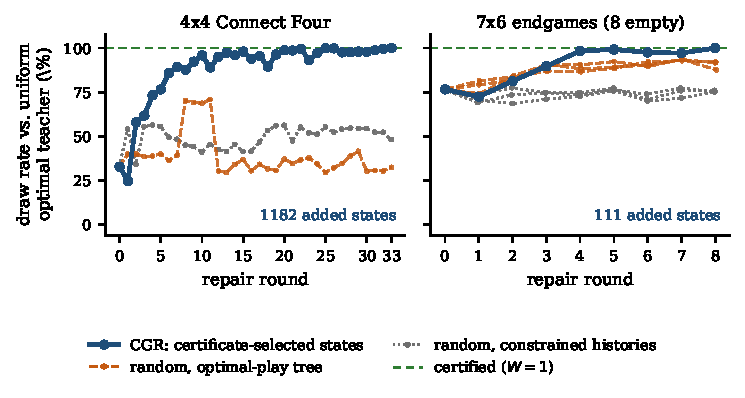
\includegraphics[width=\textwidth]{figs_v2/fig8_scaling.pdf}
\caption{Scaling the certificate and the repair at fixed model size. Left: Connect Four on $4\times4$ (base $\bar D=32.8\%$, 75 violations); 33 rounds and 1{,}182 certificate-selected histories reach $W=1$. Middle: a 40-root, eight-empty $7\times6$ endgame suite (base $\bar D=76.6\%$, 43 violations); 8 rounds and 111 histories reach $W=1$. Right: the same suite shape with ten empty cells (base $\bar D=68.2\%$, 59 violations); 17 rounds and 214 histories. Dashed and dotted lines are matched random aggregation from the optimal-play tree and from constrained histories. In every panel random controls can raise the average while leaving the worst case at zero.}
\label{fig:scaling}
\end{figure*}

\section{Certification Without a Solved Game: Hidden-Type Rock-Paper-Scissors}
\label{sec:rps}

Every experiment so far certifies a policy against a set of optimal teachers in a game with perfect information: the state is the board, the teacher's optimal set is a function of the board, and the certificate searches every tie-break. This section asks whether the diagnosis and the repair survive when the learner does not know whom it is playing, so that the object to certify is a belief rather than a tie-break set, and when the failure is a shortcut rather than a missing line.

\subsection{Game, belief, and exact certificate}
The learner plays $H=8$ rounds of Rock-Paper-Scissors against a teacher whose type $\theta\in\{0,\dots,5\}$ is hidden and fixed: always Rock, always Paper, always Scissors, copy the learner's previous action, counter it, or win-stay/lose-shift on the teacher's own previous action. Every memory type opens with Rock. The payoff is $+1$ for a win, $0$ for a tie, and $-1$ for a loss, and the learner observes actions, never the type. Its information state is therefore the history $h=((a_1,b_1),\dots,(a_k,b_k))$ of action pairs, and the set of types still possible is
\begin{equation}
\label{eq:types}
T(h) \;=\; \{\theta : \theta \text{ reproduces } b_1,\dots,b_k\}.
\end{equation}
The prior over types is uniform, so the posterior is uniform over $T(h)$. Let $b_\theta(h)$ be the teacher's next action under type $\theta$. The Bayes-adaptive value \cite{duff2002} satisfies
\begin{equation}
\label{eq:bayes}
\begin{aligned}
V^{\star}(h) \;=\; \max_{a}\;\frac{1}{|T(h)|}\sum_{\theta\in T(h)}
\bigl[&r\bigl(a,b_\theta(h)\bigr)\\
&+ V^{\star}\bigl(h,(a,b_\theta(h))\bigr)\bigr],
\end{aligned}
\end{equation}
with $V^{\star}(h)=0$ when $|h|=H$, where $Q^{\star}(h,a)$ denotes the bracketed quantity. Let $V_{\min}(h)$ be the same quantity without the maximum. For a deterministic learner $\pi$ the certificate is
\begin{equation}
\label{eq:rpscert}
\hat V(\pi) \;=\; \frac{V^{\pi}(\emptyset)-V_{\min}(\emptyset)}{V^{\star}(\emptyset)-V_{\min}(\emptyset)}
\;\in\;[0,1],
\end{equation}
where $V^{\pi}$ is \eqref{eq:bayes} evaluated at $\pi$'s actions. Because $\pi$ is deterministic and the horizon is finite, both $V^{\pi}$ and $V^{\star}$ are exact finite sums over the six types: $\hat V=1$ exactly when $\pi$ is Bayes-optimal at every history it can reach.

At the root $V^{\star}=7.000$, $V_{\min}=-7.333$, and the span is $14.333$. The root $Q$-values are $(6.333,\,7.000,\,5.667)$, so the unique Bayes-optimal opening is Paper. A clairvoyant learner that knew the type would score $8$ against every type; the canonical Bayes-optimal learner, which does not, scores $(6,7,6,8,7,8)$ against the six types, and that vector averages to $7$. The game has 19{,}234 reachable histories, 3{,}280 of them learner histories in the COPY tree, and only 34 in the tree of a Bayes-optimal policy.

\subsection{The training shortcut}
The base policy is a 64-unit GRU with 8-dimensional embeddings, trained on the 3{,}280 learner histories of the COPY tree with soft targets uniform over the exact Bayes-optimal action set, and it fits all 3{,}280 decisions. On this tree the teacher's action after round $k$ is the learner's own action at round $k-1$. The teacher tokens in the input are therefore a deterministic function of the learner tokens, so conditional on the learner's own moves the target is determined: the training signal contains nothing that rewards using the teacher channel. A model can fit all 3{,}280 decisions while ignoring it, and the base's behavior is consistent with exactly that. It scores the maximum of $8$ against COPY and also against win-stay/lose-shift, but $0$, $1$, and $-2$ out of $8$ against the three constant types and $1$ against COUNTER (\Cref{tab:rpsbase}). Its certificate is $\hat V=0.698$--$0.709$ over three seeds, with 19--20 violating frontier histories.

This is the same failure as in the solved games, with the roles of the variables changed. There, the training distribution contained one tie-break of an equivalence class; here, it contains one type, and that type's actions are \emph{redundant} given the learner's own actions. The training inputs made the hidden variable predictable on the training slice, so the network never had to use it. Off that slice---against a teacher whose action does not depend on the learner's previous move---its response is arbitrary. The analogue of sampling the optimal-teacher class is not sampling more tie-breaks of COPY; it is certifying against the belief over all types, which \eqref{eq:rpscert} does exactly.

\begin{table}[t]
\centering
\caption{Hidden-type RPS, base policy. $\hat V$ is the exact certificate of \eqref{eq:rpscert}; per-type scores are the total payoff over eight rounds against each hidden type (maximum 8). Three seeds, identical training data and budget.}
\label{tab:rpsbase}
\setlength{\tabcolsep}{3pt}
\footnotesize
\begin{tabular}{@{}lcccccccc@{}}
\toprule
\textbf{Seed} & $\hat V$ & \textbf{R} & \textbf{P} & \textbf{S} & \textbf{copy} & \textbf{cnt.} & \textbf{wsls} & \textbf{Viol.} \\
\midrule
0 & 0.698 & 0 & 1 & $-2$ & 8 & 1 & 8 & 19 \\
1 & 0.709 & 0 & 1 & $-1$ & 8 & 1 & 8 & 19 \\
2 & 0.698 & 0 & 0 & $-1$ & 8 & 1 & 8 & 20 \\
\bottomrule
\end{tabular}
\end{table}

\subsection{Bayes frontier sufficiency}
The certificate of \eqref{eq:rpscert} walks the histories that $\pi$ actually reaches when the teacher is any type still consistent with the history. Call this set $R(\pi)$; it is the analogue of the frontier of \Cref{lem:frontier}. The same sufficiency argument holds.

\begin{proposition}[Bayes frontier sufficiency]
\label{prop:rpsfrontier}
If $\pi(h)\in\arg\max_a Q^{\star}(h,a)$ for every $h\in R(\pi)$, then $V^{\pi}(\emptyset)=V^{\star}(\emptyset)$, that is, $\hat V(\pi)=1$.
\end{proposition}

\begin{proof}
Induct on the remaining depth $H-|h|$ for $h\in R(\pi)$. At $|h|=H$ both values are zero. For $|h|<H$, every successor $h'=(h,(\pi(h),b_\theta(h)))$ with $\theta\in T(h)$ is in $R(\pi)$, so by induction $V^{\pi}(h')=V^{\star}(h')$. Hence
$V^{\pi}(h)=Q^{\star}(h,\pi(h))=\max_a Q^{\star}(h,a)=V^{\star}(h)$.
The equality propagates to the root.
\end{proof}

\begin{proposition}[Progress]
\label{prop:rpsprogress}
If the aggregate $\mathcal{A}$ is fitted exactly and $\hat V(\pi)<1$, then $R(\pi)\setminus\mathcal{A}$ contains a history at which $\pi$ is not optimal. Hence every non-terminal CGR round adds at least one new history, and the loop terminates.
\end{proposition}

\begin{proof}
If $\pi$ were optimal on all of $R(\pi)$, \Cref{prop:rpsfrontier} would give $\hat V=1$. So some $h\in R(\pi)$ is non-optimal. It cannot be in $\mathcal{A}$, because the fit reaches zero aggregate regret. The aggregate is a subset of the 19{,}234 reachable histories, so it cannot grow forever.
\end{proof}

\subsection{Repair}
\Cref{tab:rpsrepair} applies the same loop with the same protocol as in the solved games: add the violating frontier histories with exact targets, oversample them $40\times$, refit the same network, and stop only when both the 3{,}280-history replay and the aggregate are exactly optimal. Across the three seeds the loop adds 53, 39, and 47 histories in seven, five, and five rounds, closes at $\hat V=1$ with zero replay mistakes, and ends at the per-type vector $(6,7,6,8,7,8)$, the Bayes optimum. No trajectory is monotone: seed 0 rises to $0.977$, falls to $0.884$ when a refit trades away one type, recovers to $0.988$, and dips to $0.942$ before closing; seed 1 falls from $0.965$ to $0.895$; seed 2 falls from the base's $0.698$ to $0.651$ after the first refit. The certificate catches each regression at the next round and the following refits repair it. Independent verification reloads each saved checkpoint and recomputes $\hat V=1$, checks that the certificate value equals a direct simulation against the six types, and checks that every aggregate history is optimal.

The selected states are 0.20--0.28\% of the reachable history space. As in every earlier domain, the states that decide robustness are a vanishing fraction of the space, and they are named by the certificate.

\subsection{Matched baselines}
\Cref{tab:rpsbase} showed that the base is not Bayes-optimal. The question is whether the repair is doing anything that random aggregation or a standard on-policy baseline could not do with the same budget. We ran five families of baselines with the same per-round added-history counts, optimizer, epochs, and stopping rule: random states from the COPY tree, from all 19{,}234 histories, and from the 34-state Bayes-optimal tree---the strongest random control, since those are the states a Bayes-optimal policy itself visits; and DAgger \cite{ross2011} with states from the learner's own rollouts against all six types, or against the worst-scoring type. Each family has three seeds. \Cref{tab:rpsctrl} reports the final certificate and \Cref{fig:rps} plots every curve.

\begin{table}[t]
\centering
\caption{Certificate-guided repair on hidden-type RPS. ``Added'' counts the certificate-selected histories, ``rounds'' the refits; every final policy is exactly Bayes-optimal and has zero replay mistakes.}
\label{tab:rpsrepair}
\setlength{\tabcolsep}{3pt}
\footnotesize
\begin{tabular}{@{}lcccccl@{}}
\toprule
\textbf{Seed} & \textbf{Before $\hat V$} & \textbf{Viol.} & \textbf{Added} & \textbf{Rounds} & \textbf{After $\hat V$} & \textbf{Final per-type} \\
\midrule
0 & 0.698 & 19 & 53 & 7 & 1.000 & $(6,7,6,8,7,8)$ \\
1 & 0.709 & 19 & 39 & 5 & 1.000 & $(6,7,6,8,7,8)$ \\
2 & 0.698 & 20 & 47 & 5 & 1.000 & $(6,7,6,8,7,8)$ \\
\bottomrule
\end{tabular}
\end{table}

\begin{table}[t]
\centering
\caption{Matched baselines on hidden-type RPS (seed 0). Same per-round counts, optimizer, epochs, and exact stopping rule as CGR; three seeds per family. Ranges are [min, max] where they differ; ``cert.'' counts runs reaching $\hat V=1$. The optimal-tree and DAgger-worst pools saturate at 34 and 43 histories.}
\label{tab:rpsctrl}
\setlength{\tabcolsep}{3pt}
\footnotesize
\begin{tabular}{@{}lcccl@{}}
\toprule
\textbf{Method} & \textbf{Added} & \textbf{Final $\hat V$} & \textbf{Cert.} \\
\midrule
Random, COPY tree & 53 & 0.709 & 0/3 \\
Random, all histories & 53 & 0.748 [0.709, 0.779] & 0/3 \\
Random, optimal tree & 34 & 1.000 & 3/3 \\
DAgger, all types & 53 & 0.977 [0.965, 1.000] & 1/3 \\
DAgger, worst type & 43 & 0.969 [0.965, 0.977] & 0/3 \\
\midrule
CGR, frontier & 53 & 1.000 & 3/3 \\
\bottomrule
\end{tabular}
\end{table}

\begin{figure*}[t]
\centering
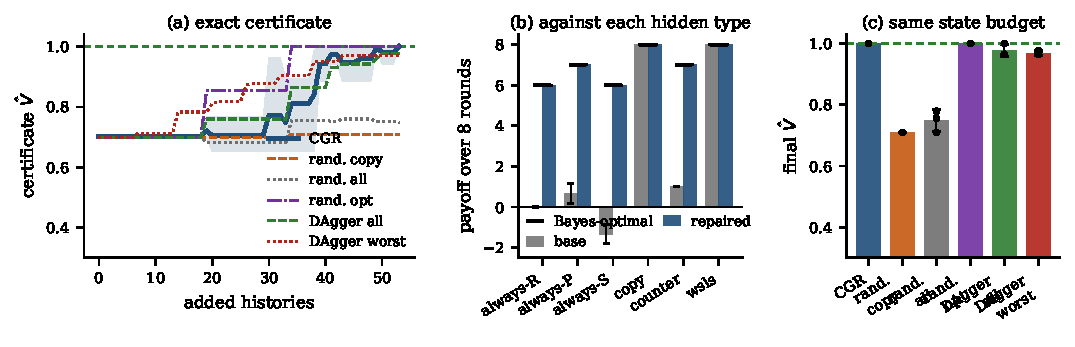
\includegraphics[width=\textwidth]{figs_v2/fig9_rps.pdf}
\caption{Hidden-type Rock-Paper-Scissors. (a) Exact certificate $\hat V$ versus added histories for CGR (three seeds, band) and five matched baselines. Random aggregation from the COPY tree or from all 19{,}234 histories stays near 0.7; DAgger and uniform sampling of the 34-history Bayes-optimal tree climb towards 1. (b) Per-type payoff, base versus repaired, with the Bayes-optimal vector as ticks; the base is maximal against COPY and WSLS and negative against Scissors. (c) Final $\hat V$ by method with individual runs; only CGR and the exhaustive optimal-tree control reach 1 in every seed.}
\label{fig:rps}
\end{figure*}

The outcome splits along one line: whether the training states come from the distribution the learner actually reaches. Uniform sampling of the COPY tree and of the full history space stays at $\hat V=0.709$--$0.779$ in all six runs. The optimal tree, in contrast, has 34 histories---the size of a frontier in this game---so two matched rounds cover it exhaustively and the policy certifies in all three seeds. DAgger, which queries the learner's own rollout distribution, lands in between: against all six types it certifies in one of three seeds ($0.965$ in the other two), and the worst-type variant, which visits only seven states per round and saturates at 43 histories, stalls at $0.965$--$0.977$, two to three points short of the optimum on COUNTER. CGR certifies every seed with 53 histories, the same per-round budget, and it is the only arm that both samples the learner's reachable states and closes the exact test in all three.

The optimal-tree result is a caveat, not a counterexample. Its pool is small enough to be covered completely, which is what the certificate says a frontier is: 34 histories whose actions determine the value. The same control fails in Tic-Tac-Toe, where the optimal-play tree has 5{,}097 histories and a matched budget of seven cannot cover it (Section~\ref{sec:repair}). The 34 states visit 7 of the 12 beliefs that occur in this game, including all four beliefs at which the base errs, so the tree corrects each violation's belief class even though only 4 of the 19 violating histories are themselves in it. This is frontier sufficiency seen from the data side: the object to cover is the belief, not the history.

DAgger's near miss is informative for the same reason. It samples states the learner reaches under one rollout distribution, while the certificate's frontier mixes types according to the current belief; rolling out only against the worst type visits seven states per round and never contains the cross-type states that decide the COUNTER payoff. Three seeds are too few to rank CGR above DAgger statistically, and we do not: at this scale, a sampler that covers a 34-state frontier can match an exact selector. What CGR provides is that its states are the ones the certificate names, so the same budget closes the exact test in every seed.

\subsection{What transfers}
The certificate here is exact for the Bayesian objective: it is the value of the policy under the true uniform prior over types, not a worst case over an adversary. That is the right object when the type is drawn from a known set and the learner cannot observe it, and it is the only exact object available at this scale; a robust or adversarial objective would require a different oracle and a different normalizer. The type set is small and hand-designed, the horizon is short, and the Bayes recursion is feasible only because there are 19{,}234 states. What the experiment does establish is narrower and, we think, more important: the diagnosis---a training distribution that makes the hidden variable redundant---and the repair---certificate-selected states on the policy's own frontier---are not tied to tie-breaking, to perfect information, or to a solved game. They transfer to a hidden-parameter game with an exact Bayes oracle, three seeds, matched random controls, and two DAgger baselines. The baselines also locate the boundary. When a frontier has 34 states, a sampler that covers it---uniform sampling of the whole optimal tree in every seed, DAgger in one of three---can match exact selection; in Tic-Tac-Toe and Connect Four the matched budgets cannot cover pools of thousands and sampling there never certifies. At this scale the certificate's value is exact selection and an exact stopping test, not sample efficiency.

\section{Audit of the Original Study}
\label{sec:audit}

The original study reported several headline phenomena. We audited each against the preserved artifacts and fresh runs. \Cref{tab:audit} summarizes the outcome; the details follow.

\begin{table*}[t]
\centering
\caption{Audit of the original claims. ``Status'' is our assessment after re-execution and reanalysis.}
\label{tab:audit}
\setlength{\tabcolsep}{3pt}
\small
\begin{tabular}{@{}>{\raggedright\arraybackslash}p{0.18\textwidth}>{\raggedright\arraybackslash}p{0.24\textwidth}>{\raggedright\arraybackslash}p{0.44\textwidth}@{}}
\toprule
\textbf{Original claim} & \textbf{Original evidence} & \textbf{Audit finding and status} \\
\midrule
100\% draw vs.\ optimal M6 & 200/200 games, one deterministic line & True but uninformative: the deterministic mentor repeats one line, so the effective sample size is one. \textbf{Ceiling only.} \\
\addlinespace
Collapse vs.\ stochastic play & GRU wins 11\% vs.\ ``random''; only D collapses & The ``random'' opponent was a greedy depth-0 solver, not uniform random. Against true uniform random the GRU wins 71\% and A/B/C/D win 55--80\%. \textbf{Retracted and corrected.} \\
\addlinespace
ACT is $2.45\times$ slower & 4{,}426\,s vs.\ 1{,}807\,s, one run & Rerun: 961\,s vs.\ 1{,}206\,s ($0.80\times$). Per-seed times range from 521 to 4{,}283\,s. \textbf{Not robust.} \\
\addlinespace
C beats A 100--0, RPS cycle & 200/200 deterministic wins & The head-to-head result is real for two deterministic lines, but there is no cycle: Random does not beat C (C wins 71\% and draws 7.5\% vs.\ uniform random). \textbf{Cycle retracted.} \\
\addlinespace
TTT to Connect Four transfer & 24/30 vs.\ 7/30 & Numerically reproducible with disjoint Wilson intervals, but one seed and different training budgets (2{,}000 vs.\ 3{,}000 games). \textbf{Suggestive, not causal.} \\
\addlinespace
Latent-geometry diagnostics & 5--7 states, coverage 12.5\% & Diagnostics have 5--7 unique boards; the equivariance ``hash'' control is tautological and the legibility probe leaks across the train/test split. \textbf{Unsupported.} \\
\bottomrule
\end{tabular}
\end{table*}

\subsection{The ``random'' baseline was not random}
The most consequential error is a mislabeled opponent. The original evaluation called \texttt{StochasticMinimax(depth=0)} ``random.'' At depth 0 the solver returns the first legal action after a 5\% exploration draw; it is a greedy, blocking opponent, not a uniform-random one. This single label error produced the ``false-master'' and ``collapse against stochastic opponents'' narratives.

We replaced the opponent with a true uniform-random \texttt{RandomAgent} and re-evaluated the preserved checkpoints. The corrected win rates are 65.5\% (A), 55.0\% (B), 71.0\% (C), and 80.0\% (D), not 96\%, 94\%, 11\%, and 7\%. The GRU agent, far from collapsing, is one of the strongest agents against uniform random play. The original claim that the agents ``collapse catastrophically when confronted with stochastic opponents'' is therefore reversed for A--C. The twin-mentor gap, by contrast, is measured against equally strong and \emph{optimal} opponents, and it replicates.

\subsection{Seed variance}
The original architectural claims rest on single runs. The preserved multi-seed data show why that is unsafe: across five seeds, A's win rate against the greedy depth-0 opponent ranges from 3\% to 90\% (mean 21.8\%, median 5\%); across four seeds, C ranges from 1\% to 96\% (mean 27.25\%, median 6\%). The two distributions overlap almost completely (\Cref{fig:seeds}). No single-run difference between A and C can be attributed to the architecture. The original paper's 96\% and 11\% are two points from these wide distributions, not stable properties.

\begin{figure}[t]
\centering
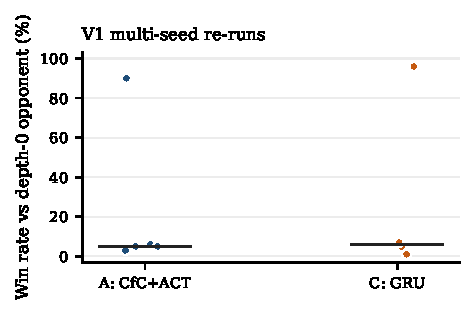
\includegraphics[width=0.92\columnwidth]{figs_v2/fig4_seeds.pdf}
\caption{V1 multi-seed win rates against the greedy depth-0 opponent that the original study called ``random.'' Each point is a seed; the black bar is the median. The same architecture spans almost the full range, so single-run architectural differences do not survive.}
\label{fig:seeds}
\end{figure}

\subsection{ACT timing}
The hardware paradox was based on one A/B pair (73m45s vs.\ 30m07s, $2.45\times$). A rerun with the same protocol gives 16m01s for A and 20m05s for B, \ie $0.80\times$: A is faster. The per-seed times in the original multi-seed data range from 521 to 4{,}283 seconds, which is larger than the A--B difference. At this scale, CPU wall-clock time is dominated by machine load and Python overhead, not by the asymptotic cost of ACT. We withdraw the hardware-paradox claim; a controlled latency benchmark with repeated runs would be required to make it.

\subsection{Non-transitivity}
The deterministic tournament does contain a striking result: C defeats A in all 200 games. But this is a comparison of two deterministic policies on two repeated lines, and it does not form a Rock-Paper-Scissors cycle. The original cycle used ``Random beats C'' based on C's 89\% draw rate against the greedy depth-0 opponent, treating draws as wins for Random. With a true uniform-random opponent, C wins 71\% and draws 7.5\%, so Random does not beat C. The correct statement is narrower: deterministic head-to-head scores between narrow policies can be extremely asymmetric, and should not be read as absolute strength. The cycle is retracted.

\subsection{Diagnostics and what survives}
The latent-geometry, equivariance, legibility, fragility-curve, and purpose probes were run on 5--7 unique boards (or one repeated line) with effective sample sizes of 1--7. The equivariance ``control'' used the agent's own decisions to define the hash, making the comparison tautological; the legibility probe split by game rather than by board, leaking the same boards into train and test. These diagnostics cannot support claims about latent geometry. We exclude them from the v2 evidence and recommend that future work report the number of unique states, not the number of decisions.

Two original results survive and motivate this paper. First, the twin-mentor gap is real and large: the preserved A/B/C checkpoints lose 75--80.5\% of games against a randomly tie-broken twin, and our fresh runs replicate it. Second, the TTT$\to$Connect Four transfer deficit is numerically reproducible (24/30 vs.\ 7/30, disjoint Wilson intervals), although the causal story about ``geometric priors'' is not established. We report the transfer result as suggestive and do not build on it.

\section{Discussion}
\label{sec:discussion}

\subsection{The certification problem}
The twin-mentor gap exposes a general weakness in how oracle-trained agents are certified. A draw rate against the teacher measures performance on the teacher's \emph{distribution}, not on the teacher's \emph{value function}. When the teacher is deterministic, those two objects can diverge sharply: the value function is correct everywhere, but the distribution covers one tie-break and one history. A single-teacher evaluation cannot distinguish a policy that has learned the value function from one that has memorized the teacher's arbitrary choices.

The fix is not to weaken the teacher. Exact-first and exact-twin teachers have identical strength; only the tie-break differs. The fix is to certify against the value function. When the game is solved, this can be done exactly: Section~\ref{sec:worst} searches the entire optimal-teacher set and returns $W$, $B$, and $\bar D$. Sampling multiple equally strong teachers estimates $\bar D$, but the estimate says nothing about the endpoints: the fixed checkpoints have $\bar D=25\%$ and $W=0$. If an exact search is not available, sampling and decision-level regret are the practical fallback, but the result should be labeled as an estimate, not a certificate. If the teacher is used for training and its optimal action set is available, randomizing ties helps expose the learner to the class---but our results show that this alone is not enough. It can relocate the failure rather than remove it. A failed certificate is also a data-selection oracle. It names the histories on which the policy must be corrected, and those histories are few: seven for C-42, five for the full-history GRU, three for a model that loses to every optimal teacher. The repair is not a different algorithm; it is the same optimizer with a different, much smaller, policy-dependent training set.

\subsection{The representation problem}
The deeper result is that a recurrent policy in a Markov game has the wrong state. Its hidden state is a function of the ordered history, so the effective state space is the history space. In Tic-Tac-Toe that space is 74.4$\times$ larger than the board space, and a full certification suite visits 13 of 180{,}361 histories. Board-level accuracy can be perfect while history-level regret remains positive, as the full-board recurrent distillation shows. A memoryless policy removes the mismatch and, with full board coverage, is robust to every tie-break we tried.

This suggests a practical rule: if the environment is Markov and the observation is the state, do not use recurrence unless the task requires memory. If recurrence is required, train and certify on the history distribution, not on one canonical history per board. Reporting the number of unique histories is as important as reporting the number of games.

\subsection{Practical recommendations}
We recommend six reporting practices for oracle-trained agents:
\begin{enumerate}
\item Evaluate against multiple \emph{equally strong} teachers that differ only in tie-breaking, and report the twin gap alongside the same-teacher score.
\item Report decision-level regret or optimal-action rate, not only game outcomes. A 100\% draw rate against one deterministic teacher is compatible with substantial regret against another optimal teacher.
\item Report the number of unique boards and unique histories visited. A 400-game certification may contain one independent observation.
\item If the environment is Markov, prefer a memoryless policy, or verify that the recurrent policy is board-optimal across all reachable boards and histories.
\item If the teacher is an exact solver and its optimal action set is available, randomize ties as a diagnostic, but do not treat it as a guarantee. Check both the fixed and the randomized certifications.
\item When the game is solved and the learner is deterministic, compute the exact worst-case certificate over the optimal-teacher set. It is feasible at this scale (27--90 states), it turns a 100\% sample into a proof or a counterexample, and it yields an exploit when the policy fails.
\item If the certificate fails, do not stop at the negative result. Use the violating frontier histories as an aggregated training set, with exact targets, and re-certify after every round (Section~\ref{sec:repair}). In the solved games, three to seven selected histories were sufficient and matched random aggregation never certified; in the hidden-type game the frontier is small enough that exhaustive sampling of the optimal tree also works (Section~\ref{sec:rps}). On-policy sampling is not a reliable substitute: matched DAgger fails in Tic-Tac-Toe, succeeds in two of three Connect Three seeds, and in the hidden-type game certifies one of six runs (Table~\ref{tab:dagger}).
\end{enumerate}
For approximate solvers, the same idea applies with a tolerance: sample among actions whose values are within $\epsilon$ of the maximum. The tolerance is a modeling choice and should be reported.

\subsection{Relation to self-play and larger games}
AlphaZero-style self-play already randomizes over near-equal moves through visit counts, so it is less exposed to the exact-tie problem. But many practical pipelines use a deterministic solver as a teacher, a scripted opponent, or a greedy expert. Those pipelines are exposed. TBR is most useful precisely where the teacher is an exact solver whose tie-breaking is an implementation detail---but our results say it is a diagnostic, not a cure.

The qualitative mechanism---a deterministic teacher collapses an equivalence class, and a history-dependent learner fails off the collapsed line---should carry over to larger games, but the magnitudes will differ. In large games exact ties are rare at shallow depth but common near the endgame; approximate ties are more common and must be defined by a tolerance. The history blow-up is likely worse, because move-order permutations grow combinatorially. The memoryless remedy is available whenever the observation is a sufficient state; when it is not, the right response is to make the state sufficient (include the missing information) rather than to add recurrence blindly.

\subsection{Limitations}
\textbf{Domain.} Tic-Tac-Toe, $4\times3$ Connect Three, and $4\times4$ Connect Four are solved games, the $7\times6$ experiment certifies a sampled endgame suite rather than the full game, and the Rock-Paper-Scissors experiment uses six hand-designed types with a known uniform prior. The state spaces make exhaustive evaluation possible, which is a strength for mechanism, but the magnitude of the gap in larger games is unknown. \textbf{Scale.} We train 5{,}000 games per run on a CPU with small networks. Our size controls (Section~\ref{sec:size}) show that 3.7 times more parameters leave mean history regret essentially unchanged (0.158 to 0.155--0.157) and keep $W=0$, while complete history coverage at fixed size reduces regret 30-fold but still does not certify at our budget. We cannot rule out that much larger models trained on complete data would eventually certify; our claim is that at matched size and data the teacher's tie policy is the causal lever. \textbf{Seeds.} Three seeds per RL condition and two seeds for the MLP are enough to see a 50--80 point effect but not enough for precise variance components; the exact sign-flip test with three seeds cannot reach $p<0.05$. Two of the nine fixed-trained checkpoints (C-43 and C-44) coincide behaviorally on all evaluated paths despite distinct weights, so the nine rows are not nine independent behaviors. \textbf{Teacher access.} The memoryless MLP and the coverage experiments use exact oracle labels; the RL agents do not. The MLP is a representation diagnostic, not an RL sample-efficiency claim. \textbf{Certificate scope.} The exact certificate requires a solved game with exact values and a deterministic learner; the adversarial teacher may condition its tie-breaks on the history, which is within the optimal class but stronger than any i.i.d. twin. For approximate values the certificate is relative to a tolerance that must be reported. \textbf{Exploration.} We kept the RL entropy schedule and curriculum fixed across conditions; other schedules could change the effect size. \textbf{Repair scope.} CGR requires an exact oracle and a deterministic learner, and the progress guarantee assumes that each round fits the aggregate exactly; we verify that condition but do not prove that it always holds. The final certificate is exact regardless. Repair can lower average accuracy off the frontier (C-42's history regret moves from 0.165 to 0.171), and in larger games both the frontier and the cost of certifying it grow. In Connect Three, matched DAgger certifies two of three seeds at the same budget, so at this scale CGR's advantage is exact selection and a deterministic stopping test, not dominance over on-policy sampling; the failures of DAgger at ten times the budget in Tic-Tac-Toe show that visitation is not a reliable substitute, not that it never works. \textbf{Bayesian scope.} The Rock-Paper-Scissors certificate is exact for the Bayesian objective under the stated prior, not for a worst case over types or over adaptively chosen opponents; it should be read as "optimal for the uncertainty the learner faces," not as a game-theoretic guarantee against an adversary who knows the policy.

\section{Conclusion}
\label{sec:conclusion}

We identified a certification failure in agents trained against optimal play. A deterministic teacher collapses each optimal equivalence class to one action and one history; a recurrent learner becomes optimal on that history line but fragile on the rest. In Tic-Tac-Toe the twin-mentor gap is 48.7--79.5 percentage points across nine checkpoints, survives an exact depth-9 control, and is visible at the decision level as zero regret against the fixed mentor and 0.12--0.21 regret against equally strong twins. An exact certificate over the entire optimal-teacher set shows that every fixed checkpoint has worst-case draw rate 0 and best case 1: its 100\% exact-first result is one extreme of the interval, and an equally optimal adaptive teacher beats it in six plies. Only the memoryless MLP and one of six TBR runs are worst-case robust. The failure is not a parameter-count artifact: 3.7 times more parameters do not remove the worst case, a memoryless model with 4.6 times fewer is certified, and randomized ties can certify the original recurrent model at fixed size. The effective state space is the history space---180{,}361 histories versus 2{,}423 boards---and a certification suite visits 5--13 of them, while the certificate that covers every optimal teacher visits 27--90. Teacher-side tie-break randomization is a seed lottery; adding noise does nothing. A memoryless policy trained on the 2{,}423 boards is robust to all 60 held-out optimal teachers, while a recurrent policy trained on the same boards still fails on histories. The lesson is general: certify agents against the teacher's value function over the state representation they actually use, not against one arbitrary realization of its tie-breaking. The certificate is also a repair map. Because a policy that is optimal on its own optimal-play frontier cannot lose, the frontier histories are a sufficient training set, and adding them with exact targets is enough: three to seven histories repaired all three failing models, while matched random aggregation with the same budget did not. DAgger is a real competitor at this scale---it certifies two of three Connect Three seeds at the same budget---but it fails without warning, including a Tic-Tac-Toe run that spends ten times CGR's budget and still misses the violating history. The certificate's states are the ones its test names. The same pattern holds when every board is covered: on Connect Three, 8--11 alternative histories repaired three seeds and eighteen controls failed. It also holds when the teacher's type is hidden and the object to certify is a belief rather than a tie-break set: in Rock-Paper-Scissors, a learner trained on a COPY teacher fits the training line while ignoring the teacher's actions, scores 0 of 8 against an always-Rock teacher, and is repaired to the exact Bayes optimum by the same certificate-selected states in all three seeds. Random aggregation from the learner's training tree or from the full history space stays at $\hat V\le0.78$, DAgger certifies one of six runs, and the only baseline certified in every seed is handed the entire 34-state optimal tree---which is what a frontier is at this scale. Certification and repair are two uses of the same object: the certificate says whether a policy is robust, and, when it is not, exactly which histories to teach.

\section*{Reproducibility}
All experiments use seeds reported in the text. The repository contains the training script (\texttt{src/ablation\_ttt.py}), the twin evaluation and regret oracle (\texttt{src/tbr\_eval.py}, \texttt{src/oracle.py}), the exact twin control (\texttt{src/exact\_twin\_eval.py}), the history and board probes (\texttt{src/history\_probe.py}, \texttt{src/space\_probe.py}), the memoryless control (\texttt{src/memoryless.py}), the coverage distillation (\texttt{src/distill\_oracle.py}), the history-coverage and width controls (\texttt{src/distill\_history.py}), the exact certificate (\texttt{src/worst\_case\_eval.py}), certificate-guided repair and its figure (\texttt{src/repair.py}, \texttt{src/repair\_figure.py}), the Connect Three/Connect Four oracle, repair, verifier, and figure (\texttt{src/c4\_game.py}, \texttt{src/c4\_repair.py}, \texttt{src/c4\_verify.py}, \texttt{src/c4\_figure.py}), the $7\times6$ endgame certificate and verifier (\texttt{src/c4\_endgame.py}, \texttt{src/c4\_endgame\_verify.py}), the hidden-type Rock-Paper-Scissors oracle, repair, verifier, figure, and tests (\texttt{src/rps\_game.py}, \texttt{src/rps\_repair.py}, \texttt{src/rps\_verify.py}, \texttt{src/rps\_figure.py}, \texttt{tests/test\_rps.py}), and the experiment matrix (\texttt{experiments/run\_matrix.sh}). Every evaluation records a truncated SHA-256 of the checkpoint it loaded; the preserved v1 checkpoints are in \texttt{artifacts/v1\_reentreno}. Figures are generated by \texttt{src/make\_figures.py} from the JSON files in \texttt{data/}. The paper is built with Tectonic from \texttt{paper/paper\_v2.tex}.

\begin{thebibliography}{99}

\bibitem{silver2016}
D.~Silver, A.~Huang, C.~J. Maddison, A.~Guez, L.~Sifre, G.~van~den~Driessche, J.~Schrittwieser, I.~Antonoglou, V.~Panneershelvam, M.~Lanctot, \etal, ``Mastering the game of Go with deep neural networks and tree search,'' \emph{Nature}, vol.~529, no.~7587, pp.~484--489, 2016.

\bibitem{silver2018}
D.~Silver, T.~Hubert, J.~Schrittwieser, I.~Antonoglou, M.~Lai, A.~Guez, M.~Lanctot, L.~Sifre, D.~Kumaran, T.~Graepel, T.~Lillicrap, K.~Simonyan, and D.~Hassabis, ``A general reinforcement learning algorithm that masters chess, shogi, and Go through self-play,'' \emph{Science}, vol.~362, no.~6419, pp.~1140--1144, 2018.

\bibitem{ross2011}
S.~Ross, G.~J. Gordon, and J.~A. Bagnell, ``A reduction of imitation learning and structured prediction to no-regret online learning,'' in \emph{Proc. International Conference on Artificial Intelligence and Statistics}, 2011, pp.~627--635.

\bibitem{henderson2018}
P.~Henderson, R.~Islam, P.~Bachman, J.~Pineau, D.~Precup, and D.~Meger, ``Deep reinforcement learning that matters,'' in \emph{Proc. AAAI Conference on Artificial Intelligence}, vol.~32, 2018.

\bibitem{agarwal2021}
R.~Agarwal, M.~Schwarzer, P.~S. Castro, A.~Courville, and M.~G. Bellemare, ``Deep reinforcement learning at the edge of the statistical precipice,'' in \emph{Advances in Neural Information Processing Systems}, vol.~34, 2021.

\bibitem{czarnecki2020}
W.~M. Czarnecki, G.~Gidel, B.~Tracey, K.~Tuyls, S.~Omidshafiei, D.~Balduzzi, and M.~Jaderberg, ``Real world games look like spinning tops,'' in \emph{Advances in Neural Information Processing Systems}, vol.~33, 2020, pp.~17443--17454.

\bibitem{balduzzi2019}
D.~Balduzzi, M.~Garnelo, Y.~Bachrach, W.~Czarnecki, J.~Perolat, M.~Jaderberg, and T.~Graepel, ``Open-ended learning in symmetric zero-sum games,'' in \emph{Proc. International Conference on Machine Learning}, 2019, pp.~434--443.

\bibitem{jaderberg2019}
M.~Jaderberg, W.~M. Czarnecki, I.~Dunning, L.~Marris, G.~Lever, A.~G. Casta\~{n}eda, C.~Beattie, N.~C. Rabinowitz, A.~S. Morcos, A.~Ruderman, N.~Sonnerat, T.~Green, L.~Deason, J.~Z. Leibo, D.~Silver, D.~Hassabis, K.~Kavukcuoglu, and T.~Graepel, ``Human-level performance in 3D multiplayer games with population-based reinforcement learning,'' \emph{Science}, vol.~364, no.~6443, pp.~859--865, 2019.

\bibitem{pinto2017}
L.~Pinto, J.~Davidson, R.~Sukthankar, and A.~Gupta, ``Robust adversarial reinforcement learning,'' in \emph{Proc. International Conference on Machine Learning}, 2017, pp.~2817--2826.

\bibitem{sutton1998}
R.~S. Sutton and A.~G. Barto, \emph{Reinforcement Learning: An Introduction}. Cambridge, MA: MIT Press, 1998.

\bibitem{kaelbling1998}
L.~P. Kaelbling, M.~L. Littman, and A.~R. Cassandra, ``Planning and acting in partially observable stochastic domains,'' \emph{Artificial Intelligence}, vol.~101, no.~1--2, pp.~99--134, 1998.

\bibitem{puterman1994}
M.~L. Puterman, \emph{Markov Decision Processes: Discrete Stochastic Dynamic Programming}. New York: Wiley, 1994.

\bibitem{cho2014}
K.~Cho, B.~van~Merri\"{e}nboer, C.~Gulcehre, D.~Bahdanau, F.~Bougares, H.~Schwenk, and Y.~Bengio, ``Learning phrase representations using RNN encoder-decoder for statistical machine translation,'' in \emph{Proc. Conference on Empirical Methods in Natural Language Processing}, 2014, pp.~1724--1734.

\bibitem{hasani2021}
R.~Hasani, M.~Lechner, A.~Amini, L.~Liebenwein, A.~Ray, S.~Tschaikowski, G.~Teschl, and D.~Rus, ``Closed-form continuous-time neural networks,'' in \emph{Advances in Neural Information Processing Systems}, vol.~35, 2022.

\bibitem{lanctot2017}
M.~Lanctot, V.~Zambaldi, A.~Gruslys, A.~Lazaridou, K.~Tuyls, J.~P\'{e}rolat, D.~Silver, and T.~Graepel, ``A unified game-theoretic approach to multiagent reinforcement learning,'' in \emph{Advances in Neural Information Processing Systems}, vol.~30, 2017.

\bibitem{zhang2018}
C.~Zhang, O.~Vinyals, R.~Munos, and S.~Bengio, ``A study on overfitting in deep reinforcement learning,'' \emph{arXiv preprint arXiv:1804.06893}, 2018.

\bibitem{taylor2009}
M.~E. Taylor and P.~Stone, ``Transfer learning for reinforcement learning domains: A survey,'' \emph{Journal of Machine Learning Research}, vol.~10, pp.~1633--1685, 2009.

\bibitem{wilson1927}
E.~B. Wilson, ``Probable inference, the law of succession, and statistical inference,'' \emph{Journal of the American Statistical Association}, vol.~22, no.~158, pp.~209--212, 1927.

\bibitem{efron1993}
B.~Efron and R.~J. Tibshirani, \emph{An Introduction to the Bootstrap}. New York: Chapman \& Hall, 1993.

\bibitem{damour2020}
A.~D'Amour, K.~Heller, D.~Moldovan, B.~Adlam, B.~Alayrac, A.~Beutel, C.~Chen, D.~Deaton, J.~Eisenstein, M.~D. Hoffman, \etal, ``Underspecification presents challenges for credibility in modern machine learning,'' \emph{Journal of Machine Learning Research}, vol.~23, no.~226, pp.~1--61, 2022.

\bibitem{geirhos2020}
R.~Geirhos, J.-H. Jacobsen, C.~Michaelis, R.~Zemel, W.~Breit, M.~Bethge, and F.~A. Wichmann, ``Shortcut learning in deep neural networks,'' \emph{Nature Machine Intelligence}, vol.~2, pp.~665--673, 2020.

\bibitem{duff2002}
M.~O. Duff, ``Optimal learning: Computational procedures for Bayes-adaptive Markov decision processes,'' Ph.D. dissertation, University of Massachusetts Amherst, 2002.

\end{thebibliography}

\end{document}
